\chapter{Metodologia}
Neste capítulo serão apresentados os levantamento de informações e os requisitos do trabalho. Antes de qualquer coisa devemos primeiramente entender o significado de metodologia, que nada mais é onde é permitido descrever o caminho percorrido para atingir o objetivo proposto, buscando solucionar a questão de pesquisa.

Logo também precisamos entender o que é um modelo de caso de uso, É através dele onde podemos descrever como diferentes tipos de usuários interagem com o sistema para resolver um problema. Como tal, ele descreve as metas dos usuários, as interações entre os usuários e o sistema, bem como o comportamento necessário do sistema para satisfazer estas metas.

A fim de expor detalhadamente os procedimentos e métodos que foram adotados no
estudo, foi dividido em oito tópicos.

\section{CASOS DE USO}
\subsection{CASOS DE USO: EFETUAR LOGIN}
\begin{flushleft}
\textbf{Ator:}  Proprietário
\\
\textbf{Pré-Requisito:} Ter Cadastrado Senha e Login do Funcionário.
\end{flushleft}

\begin{figure}[htb]
	\caption{\label{fig_login} Diagrama caso de uso - Efetuar Login}
	\begin{center}
	    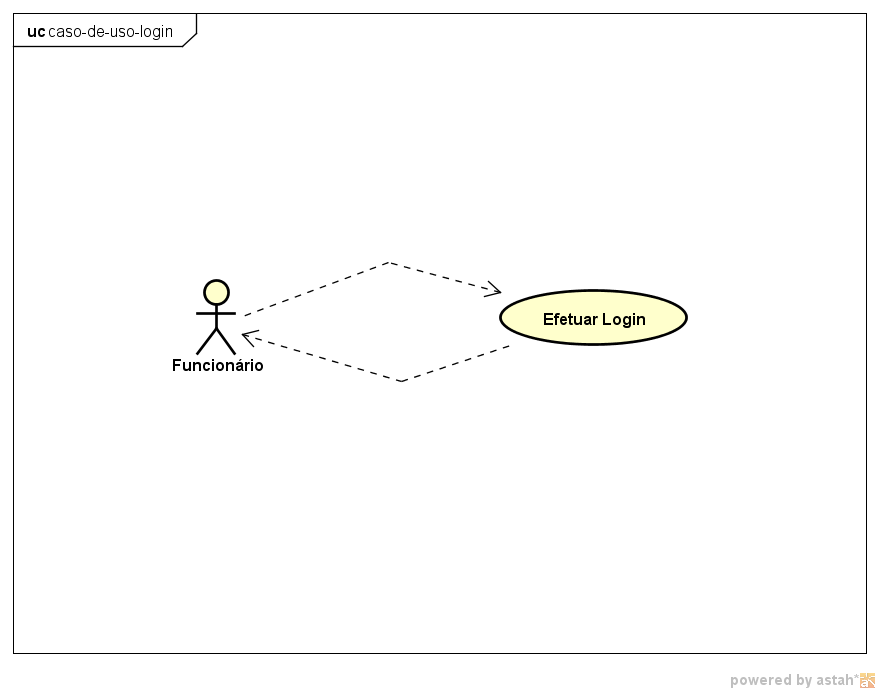
\includegraphics[width=0.7\linewidth]{imagens/caso-de-uso-login.png}
	\end{center}
\end{figure}

\newpage

\begin{table}
\begin{tabular}{l|l}
\hline
\multicolumn{1}{c|} 
{\textbf{Ação do Ator}} &
\multicolumn{1}{c}
{\textbf{Resposta do Sistema ou Exceções}} \\ \hline
\begin{tabular}[c]{@{}l@{}}1-O Usuário inicia o\\ Sistema de Ordem de\\ Serviço.\end{tabular} & \begin{tabular}[c]{@{}l@{}}2- O Sistema exibe a janela com dois campos para o\\ Usuário informar Login e Senha.\end{tabular} \\ \hline
\begin{tabular}[c]{@{}l@{}}3- O Usuário informa\\ Login, Senha e\\ Confirma.\end{tabular} & \begin{tabular}[c]{@{}l@{}}4- O Sistema faz a validação do Login e Senha\\ informada com os dados de Login e Senha\\ cadastrado no Sistema, [Passo 7].\end{tabular} \\ \hline
 & \begin{tabular}[c]{@{}l@{}}5-O Sistema abre dando acesso a todo o Sistema\\ com exceção do Funcionário que somente terá\\ acesso a tela de geração de O.S.\end{tabular} \\ \hline
\begin{tabular}[c]{@{}l@{}}6- O Usuário já pode\\ utilizar O Sistema.\end{tabular} &  \\ \hline
\begin{tabular}[c]{@{}l@{}}7-(Exceção) O Usuário\\ informa Login e Senha\\ incorretas retorna ao\\ passo 2.\end{tabular} &  \\ \hline
\end{tabular}
\caption{Caso de uso - Efetuar Login}
\end{table}

\subsection{CASOS DE USO: CADASTRAR USUÁRIO}
\begin{flushleft}
\textbf{Ator:}  Proprietário
\end{flushleft}

\begin{figure}[htb]
	\caption{\label{fig_login} Diagrama caso de uso - Cadastrar Usuário}
	\begin{center}
	    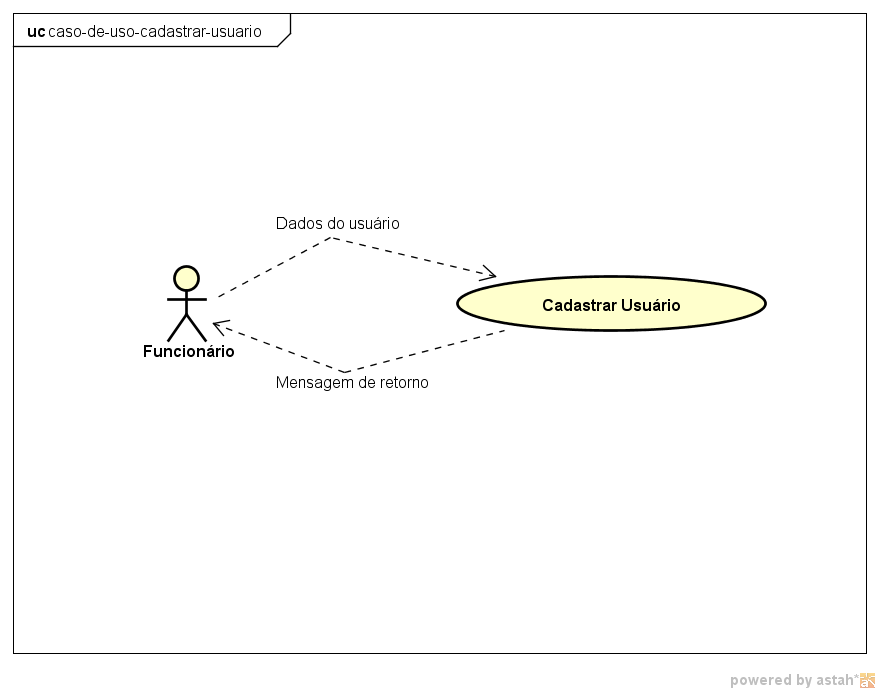
\includegraphics[width=0.7\linewidth]{imagens/cadastrar-usuario.png}
	\end{center}
\end{figure}

\newpage

\begin{table}[]
\begin{tabular}{l|l}
\hline
\multicolumn{1}{c|}{\textbf{Ação do Ator}} & \multicolumn{1}{c}{\textbf{Resposta do Sistema ou Exceções}} \\ \hline
\begin{tabular}[c]{@{}l@{}}1- O Usuário inicia solicitando a tela\\ de Login.\end{tabular} & \begin{tabular}[c]{@{}l@{}}2- O Sistema inicia abrindo a tela de\\ Login.\end{tabular} \\ \hline
\begin{tabular}[c]{@{}l@{}}3- O Usuário informa seu Login e\\ Senha ao Sistema.\end{tabular} & \begin{tabular}[c]{@{}l@{}}4- O Sistema valida a Senha e Login e\\ abre a tela inicial dando acesso a todo\\ o Sistema, [passo 9].\end{tabular} \\ \hline
\begin{tabular}[c]{@{}l@{}}5- O Usuário seleciona a tela de\\ cadastro de Usuário do Menu.\end{tabular} & \begin{tabular}[c]{@{}l@{}}6- O Sistema abre a tela de cadastro\\ de Usuário.\end{tabular} \\ \hline
\begin{tabular}[c]{@{}l@{}}7- O Usuário Proprietário entra com \\ os dados do Usuário, Nome, RG, CPF, \\ Endereço, E-mail, Telefone, Senha\end{tabular} & \begin{tabular}[c]{@{}l@{}}8- O Sistema Salva e Retorna \\ ao passo 6 .\end{tabular} \\ \hline
\begin{tabular}[c]{@{}l@{}}9- (Exceção) O Usuário informa Login \\ ou Senha Incorreta e o Sistema e \\ retorna ao passo 2.\end{tabular} & \begin{tabular}[c]{@{}l@{}}10- (Exceção) O Usuário Cancela o\\ cadastro e retorna ao passo 6.\end{tabular} \\ \hline
\begin{tabular}[c]{@{}l@{}}11- (Exceção) – O Sistema informa \\ que o CPF e o RG informado já esta sendo \\ utilizado e volta ao passo 7.\end{tabular} &  \\ \hline
\end{tabular}
\caption{Caso de uso - Cadastrar Usuário}
\end{table}

\subsection{CASOS DE USO: CADASTRAR FUNCIONÁRIO}
\begin{flushleft}
\textbf{Ator:}  Proprietário
\end{flushleft}

\begin{figure}[htb]
	\caption{\label{fig_funcionario} Diagrama caso de uso - Cadastrar Funcionário}
	\begin{center}
	    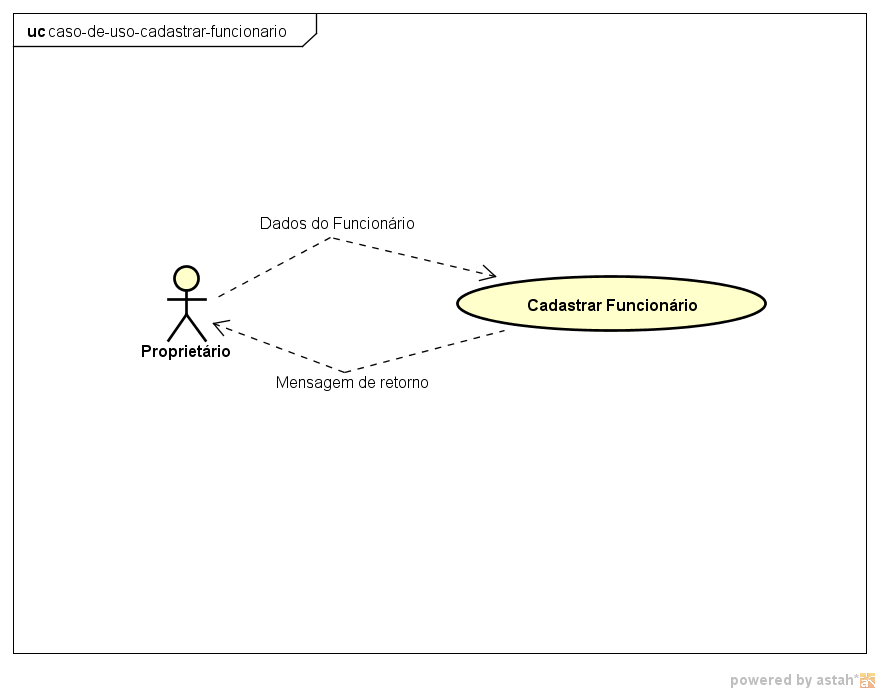
\includegraphics[width=0.7\linewidth]{imagens/cadastrar-funcionario.png}
	\end{center}
\end{figure}

\newpage

\begin{table}[]
\begin{tabular}{l|l}
\hline
\multicolumn{1}{c|}{\textbf{Ação do Ator}} & \multicolumn{1}{c}{\textbf{Resposta do Sistema ou Exceções}} \\ \hline
\begin{tabular}[c]{@{}l@{}}1- O Usuário inicia solicitando a tela\\ de Login.\end{tabular} & \begin{tabular}[c]{@{}l@{}}2- O Sistema inicia abrindo a tela de\\ Login.\end{tabular} \\ \hline
\begin{tabular}[c]{@{}l@{}}3- O Usuário informa seu Login e\\ Senha ao Sistema.\end{tabular} & \begin{tabular}[c]{@{}l@{}}4- O Sistema valida a Senha e Login e\\ abre a tela inicial dando acesso a todo\\ o Sistema, [passo 9].\end{tabular} \\ \hline
\begin{tabular}[c]{@{}l@{}}5- O Usuário seleciona a tela de\\ cadastro de Funcionário do Menu.\end{tabular} & \begin{tabular}[c]{@{}l@{}}6- O Sistema abre a tela de cadastro\\ de Funcionário.\end{tabular} \\ \hline
\begin{tabular}[c]{@{}l@{}}7- O Usuário entra com os dados do\\ Funcionário, Nome, CPF, Endereço, \\ Data de nascimento, Data de Admissão.\end{tabular} & \begin{tabular}[c]{@{}l@{}}8- O Sistema Salva e Retorna \\ ao passo 6 .\end{tabular} \\ \hline
\begin{tabular}[c]{@{}l@{}}9- (Exceção) O Usuário informa Login \\ ou Senha Incorreta e o Sistema e \\ Retorna ao passo 2.\end{tabular} & \begin{tabular}[c]{@{}l@{}}10- (Exceção) O Usuário Cancela o\\ cadastro e retorna ao passo 6.\end{tabular} \\ \hline
\begin{tabular}[c]{@{}l@{}}11- (Exceção) – O Sistema informa \\ que as Senhas não conferem e volta ao\\ passo 7.\end{tabular} &  \\ \hline
\end{tabular}
\caption{Caso de uso - Cadastrar Funcionário}
\end{table}

\subsection{CASOS DE USO: CADASTRAR CLIENTE}
\begin{flushleft}
\textbf{Ator:}  Proprietário
\end{flushleft}

\begin{figure}[htb]
	\caption{\label{fig_cliente} Diagrama caso de uso - Cadastrar Cliente}
	\begin{center}
	    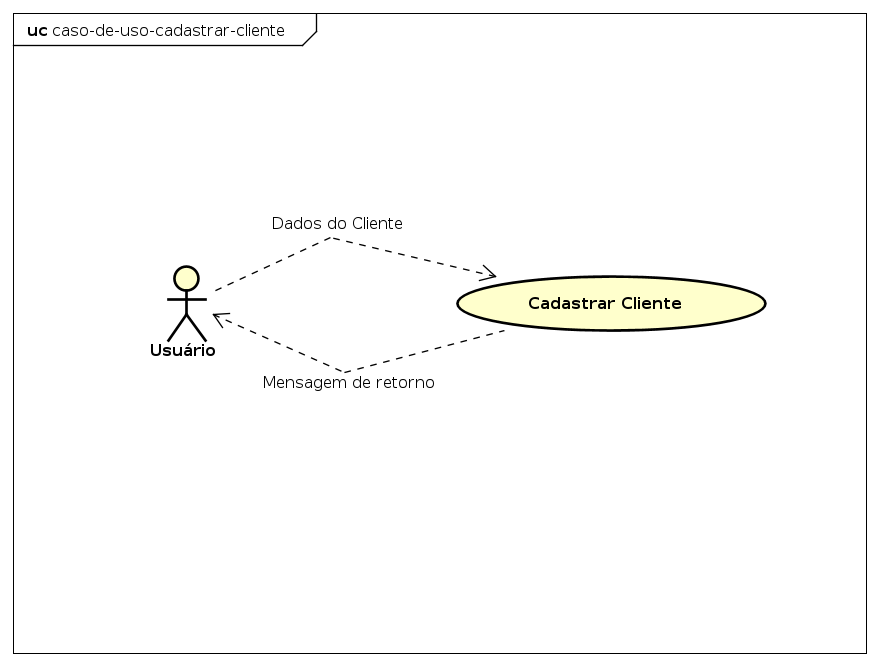
\includegraphics[width=0.7\linewidth]{imagens/cadastrar-cliente.png}
	\end{center}
\end{figure}

\newpage

\begin{table}[]
\begin{tabular}{l|l}
\hline
\multicolumn{1}{c|}{\textbf{Ação do Ator}} & \multicolumn{1}{c}{\textbf{Resposta do Sistema ou Exceções}} \\ \hline
\begin{tabular}[c]{@{}l@{}}1- O Usuário inicia solicitando a tela\\ de Login.\end{tabular} & \begin{tabular}[c]{@{}l@{}}2- O Sistema inicia abrindo a tela de\\ Login.\end{tabular} \\ \hline
\begin{tabular}[c]{@{}l@{}}3- O Usuário informa seu Login e\\ Senha ao Sistema.\end{tabular} & \begin{tabular}[c]{@{}l@{}}4- O Sistema valida a Senha e Login e\\ abre a tela inicial dando acesso a todo\\ o Sistema, [passo 9].\end{tabular} \\ \hline
\begin{tabular}[c]{@{}l@{}}5- O Usuário seleciona a tela de\\ cadastro de Cliente do Menu.\end{tabular} & \begin{tabular}[c]{@{}l@{}}6- O Sistema abre a tela de cadastro\\ de Cliente.\end{tabular} \\ \hline
\begin{tabular}[c]{@{}l@{}}7- O Usuário entra com os dados do\\ Cliente, Nome, CPF, Endereço, \\ Cidade, Estado, Telefone, E-mail\\ e Data de Nascimento\end{tabular} & \begin{tabular}[c]{@{}l@{}}8- O Sistema Salva e Retorna \\ ao passo 6 .\end{tabular} \\ \hline
\begin{tabular}[c]{@{}l@{}}9- (Exceção) O Usuário informa Login \\ ou Senha Incorreta e o Sistema e \\ Retorna ao passo 2.\end{tabular} & \begin{tabular}[c]{@{}l@{}}10- (Exceção) O Usuário Cancela o\\ cadastro e retorna ao passo 6.\end{tabular} \\ \hline
\begin{tabular}[c]{@{}l@{}}11- (Exceção) – O Sistema informa \\ que o CPF informado já esta sendo \\ utilizado e volta ao passo 7.\end{tabular} &  \\ \hline
\end{tabular}
\caption{Caso de uso - Cadastrar Cliente}
\end{table}

\subsection{CASOS DE USO: CADASTRAR SERVIÇOS}
\begin{flushleft}
\textbf{Ator:}  Proprietário
\end{flushleft}

\begin{figure}[htb]
	\caption{\label{fig_cliente} Diagrama caso de uso - Cadastrar Serviços}
	\begin{center}
	    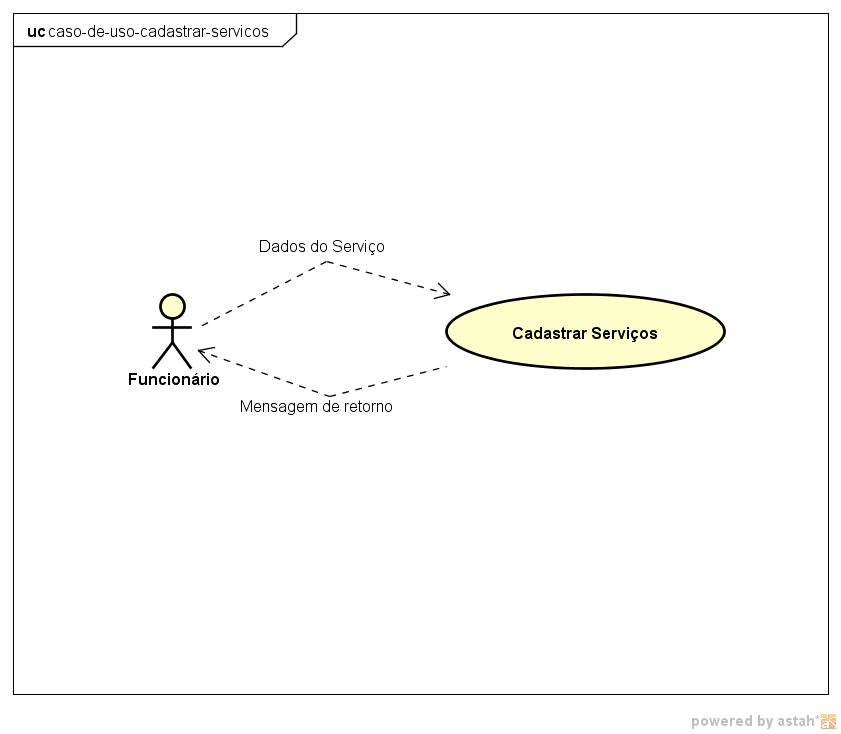
\includegraphics[width=0.6\linewidth]{imagens/cadastrar-servico.png}
	\end{center}
\end{figure}

\newpage

\begin{table}[]
\begin{tabular}{l|l}
\hline
\multicolumn{1}{c|}{\textbf{Ação do Ator}} & \multicolumn{1}{c}{\textbf{Resposta do Sistema ou Exceções}} \\ \hline
\begin{tabular}[c]{@{}l@{}}1- O Usuário inicia solicitando a tela\\ de Login.\end{tabular} & \begin{tabular}[c]{@{}l@{}}2- O Sistema inicia abrindo a tela de\\ Login.\end{tabular} \\ \hline
\begin{tabular}[c]{@{}l@{}}3- O Usuário informa seu Login e\\ Senha ao Sistema.\end{tabular} & \begin{tabular}[c]{@{}l@{}}4- O Sistema valida a Senha e Login e\\ abre a tela inicial dando acesso a todo\\ o Sistema, [passo 9].\end{tabular} \\ \hline
\begin{tabular}[c]{@{}l@{}}5- O Usuário seleciona a tela de\\ cadastro de Serviços do Menu.\end{tabular} & \begin{tabular}[c]{@{}l@{}}6- O Sistema abre a tela de cadastro\\ de Serviços.\end{tabular} \\ \hline
\begin{tabular}[c]{@{}l@{}}7- O Usuário entra com \\ os dados do Serviço, Descrição do serviço\\ e valor do serviço.\end{tabular} & \begin{tabular}[c]{@{}l@{}}8- O Sistema Salva e Retorna \\ ao passo 6 .\end{tabular} \\ \hline
\begin{tabular}[c]{@{}l@{}}9- (Exceção) O Usuário informa Login \\ ou Senha Incorreta e o Sistema e \\ retorna ao passo 2.\end{tabular} & \begin{tabular}[c]{@{}l@{}}10- (Exceção) O Usuário Cancela o\\ cadastro e retorna ao passo 6.\end{tabular} \\ \hline
\end{tabular}
\caption{Caso de uso - Cadastrar Serviços}
\end{table}

\subsection{CASOS DE USO: CADASTRAR ORDEM DE SERVIÇO}
\begin{flushleft}
\textbf{Ator:}  Proprietário
\\
\textbf{Pré-Requisito:} Ter cadastrado o cliente, funcionário e o serviço.
\end{flushleft}

\begin{figure}[htb]
	\caption{\label{fig_cliente} Diagrama caso de uso - Cadastrar Ordem de Serviço}
	\begin{center}
	    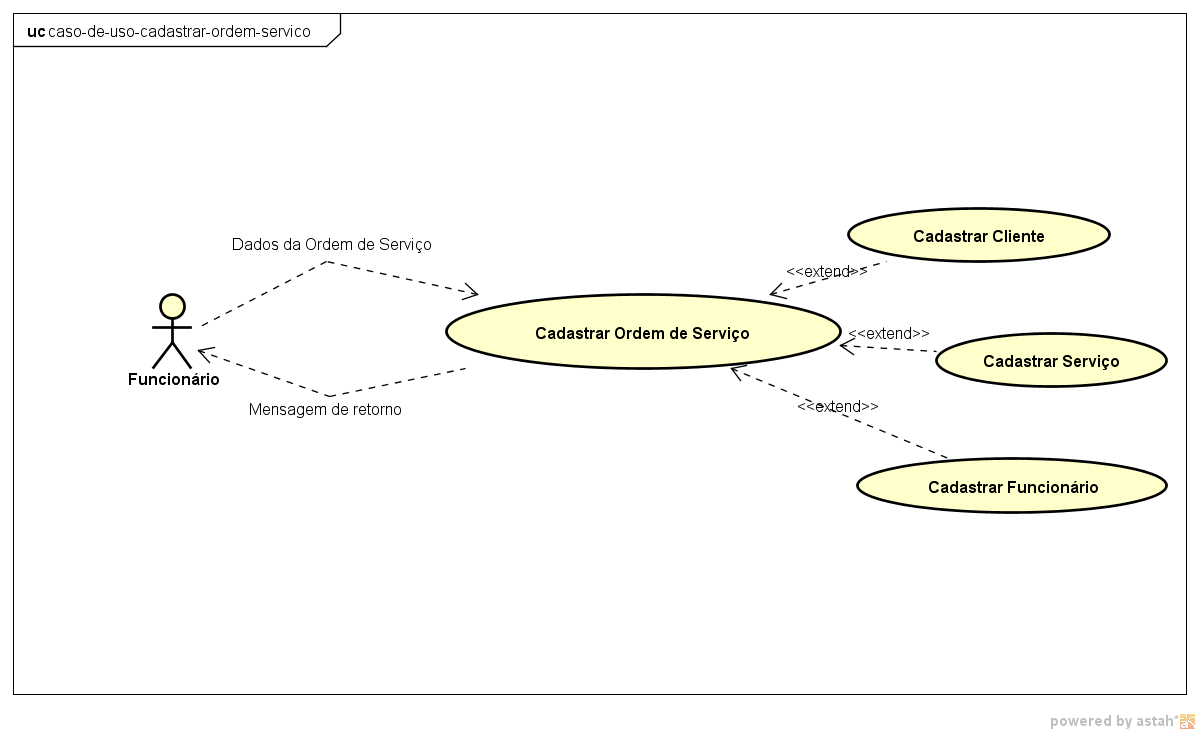
\includegraphics[width=0.7\linewidth]{imagens/cadastrar-ordem-de-servico.png}
	\end{center}
\end{figure}

\newpage

\begin{table}[]
\begin{tabular}{l|l}
\hline
\multicolumn{1}{c|}{\textbf{Ação do Ator}} & \multicolumn{1}{c}{\textbf{Resposta do Sistema ou Exceções}} \\ \hline
\begin{tabular}[c]{@{}l@{}}1- O Usuário inicia solicitando a tela\\ de Login.\end{tabular} & \begin{tabular}[c]{@{}l@{}}2- O Sistema inicia abrindo a tela de\\ Login.\end{tabular} \\ \hline
\begin{tabular}[c]{@{}l@{}}3- O Usuário informa seu Login e\\ Senha ao Sistema.\end{tabular} & \begin{tabular}[c]{@{}l@{}}4- O Sistema valida a Senha e Login e\\ abre a tela inicial dando acesso a todo\\ o Sistema, [passo 9].\end{tabular} \\ \hline
\begin{tabular}[c]{@{}l@{}}5- O Usuário seleciona a tela de\\ cadastro de Ordem de Serviço do Menu.\end{tabular} & \begin{tabular}[c]{@{}l@{}}6- O Sistema abre a tela de cadastro\\ de Ordem de Serviço.\end{tabular} \\ \hline
\begin{tabular}[c]{@{}l@{}}7- O Usuário entra informa qual o cliente,\\ funcionário e o serviço.\end{tabular} & \begin{tabular}[c]{@{}l@{}}8- O Sistema Salva e Retorna \\ ao passo 6 .\end{tabular} \\ \hline
\begin{tabular}[c]{@{}l@{}}9- (Exceção) O Usuário informa Login \\ ou Senha Incorreta e o Sistema e \\ retorna ao passo 2.\end{tabular} & \begin{tabular}[c]{@{}l@{}}10- (Exceção) O Usuário Cancela o\\ cadastro e retorna ao passo 6.\end{tabular} \\ \hline
\end{tabular}
\caption{Caso de uso - Cadastrar Ordem de Serviço}
\end{table}

\section{DIAGRAMA DE ATIVIDADES}
\subsection{VISÃO GERAL}
\begin{figure}[htb]
	\caption{\label{fig_visao-geral} Diagrama de Atividades - Visão Geral do Sistema}
	\begin{center}
	    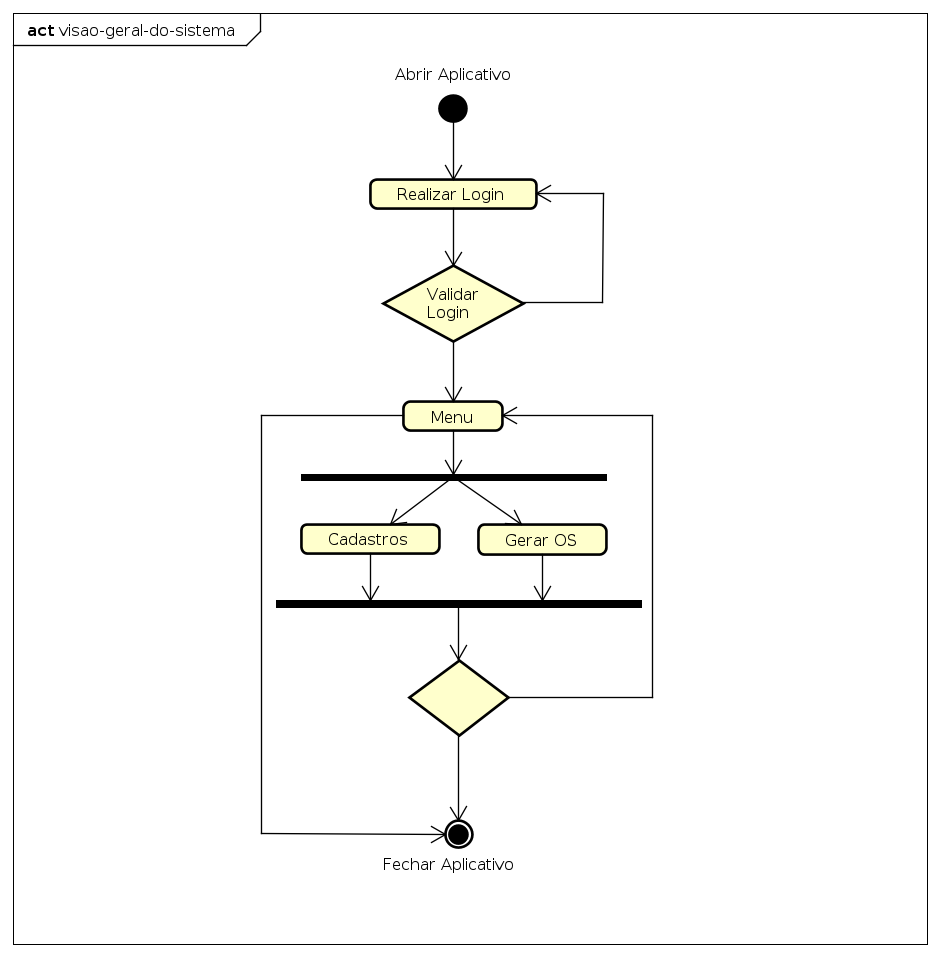
\includegraphics[width=0.7\linewidth]{imagens/diagrama-atividade-visao-geral.png}
	\end{center}
\end{figure}

\newpage

\subsection{CADASTROS}
\begin{figure}[htb]
	\caption{\label{fig_cadastro} Diagrama de Atividades - Cadastro do Sistema}
	\begin{center}
	    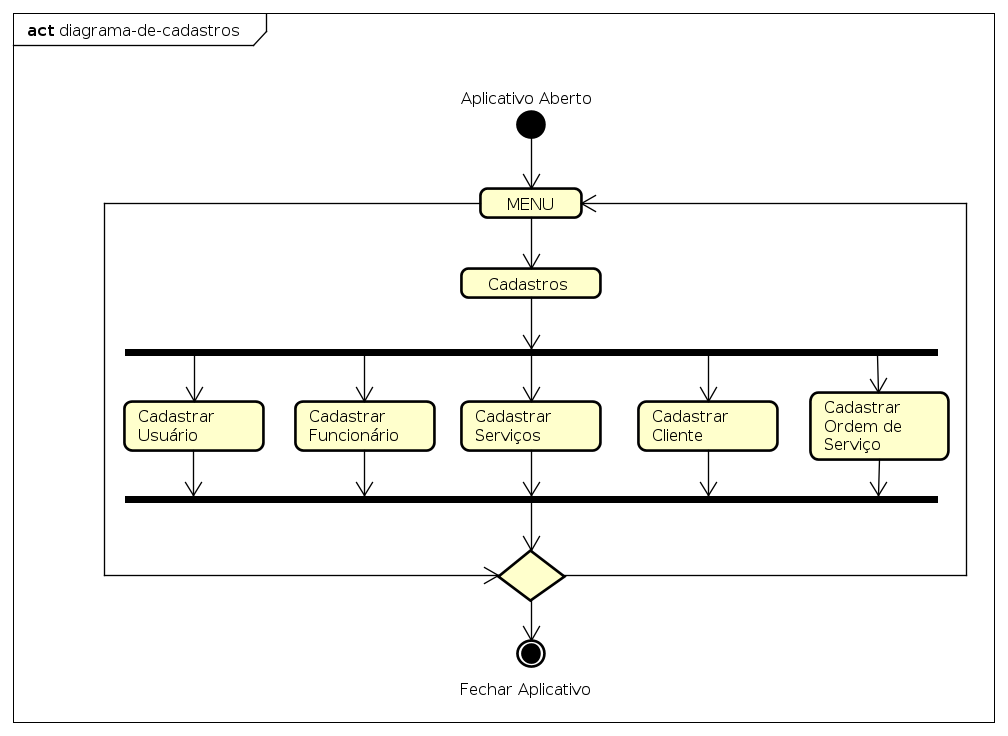
\includegraphics[width=0.9\linewidth]{imagens/diagrama-de-cadastros.png}
	\end{center}
\end{figure}

\subsubsection{CADASTRAR USUÁRIO}
\begin{figure}[htb]
	\caption{\label{fig_cadastro} Diagrama de Atividades - Cadastro do Sistema}
	\begin{center}
	    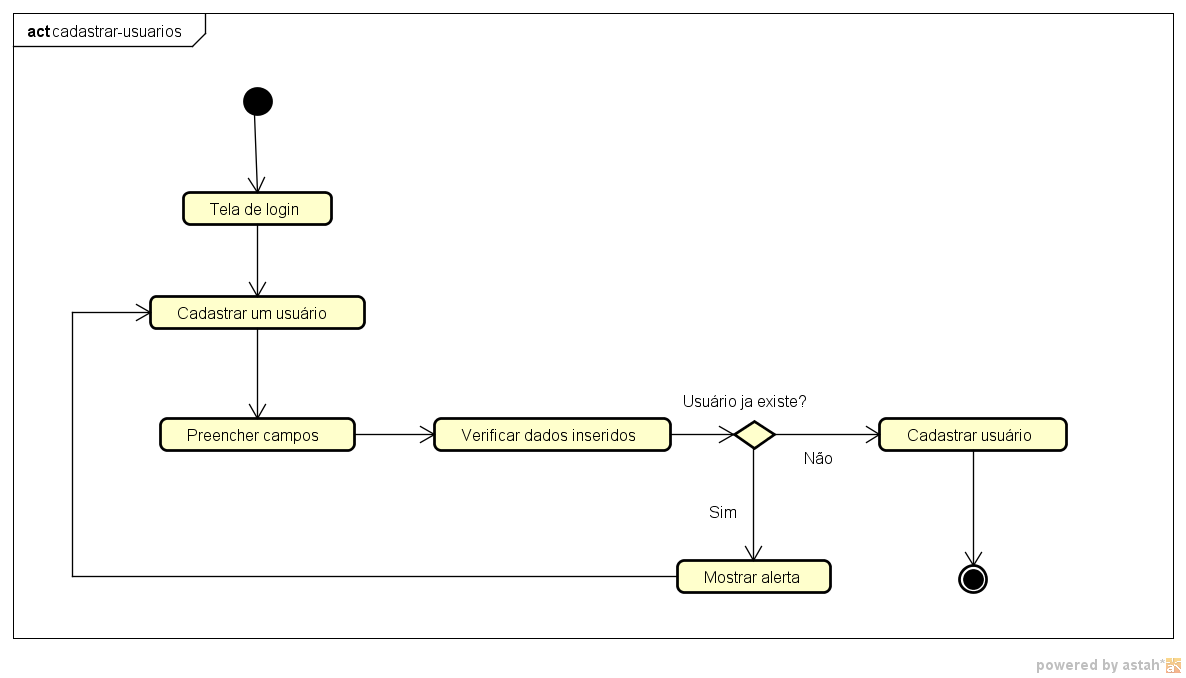
\includegraphics[width=0.8\linewidth]{imagens/usuarios.png}
	\end{center}
\end{figure}

\newpage

\subsubsection{CADASTRAR FUNCIONÁRIO}
\begin{figure}[htb]
	\caption{\label{fig_cadastro} Diagrama de Atividades - Cadastro do Sistema}
	\begin{center}
	    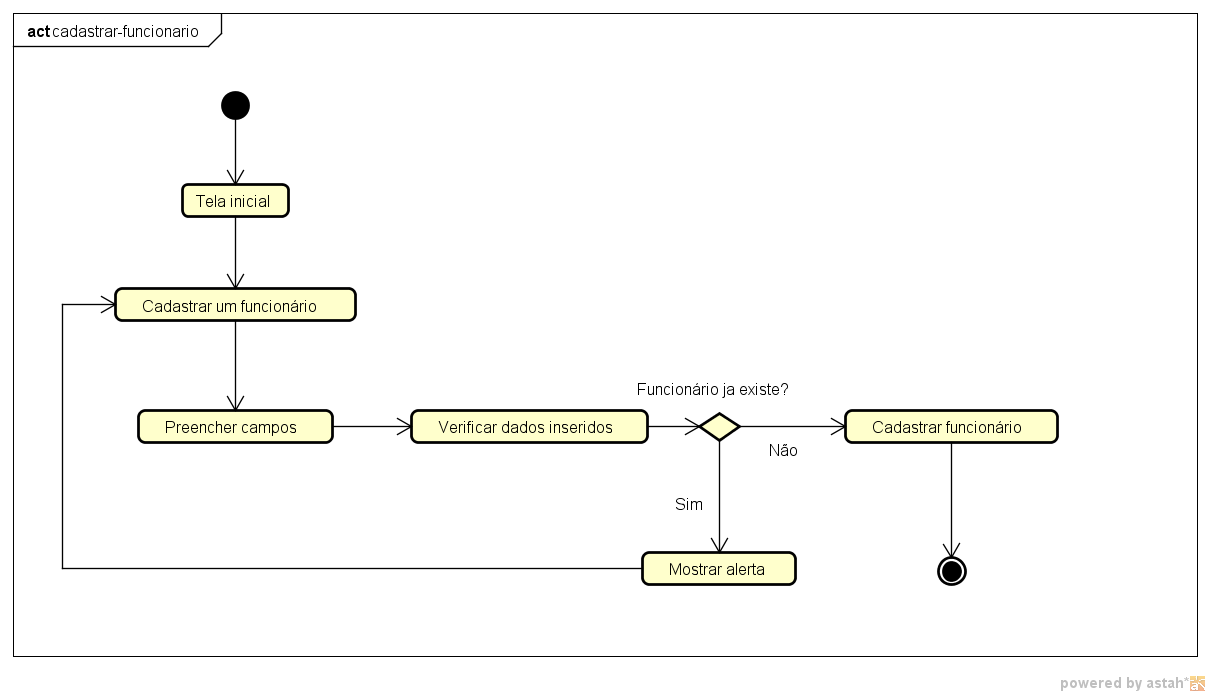
\includegraphics[width=0.8\linewidth]{imagens/funcionario.png}
	\end{center}
\end{figure}

\subsubsection{CADASTRAR SERVIÇOS}
\begin{figure}[htb]
	\caption{\label{fig_cadastro} Diagrama de Atividades - Cadastro do Sistema}
	\begin{center}
	    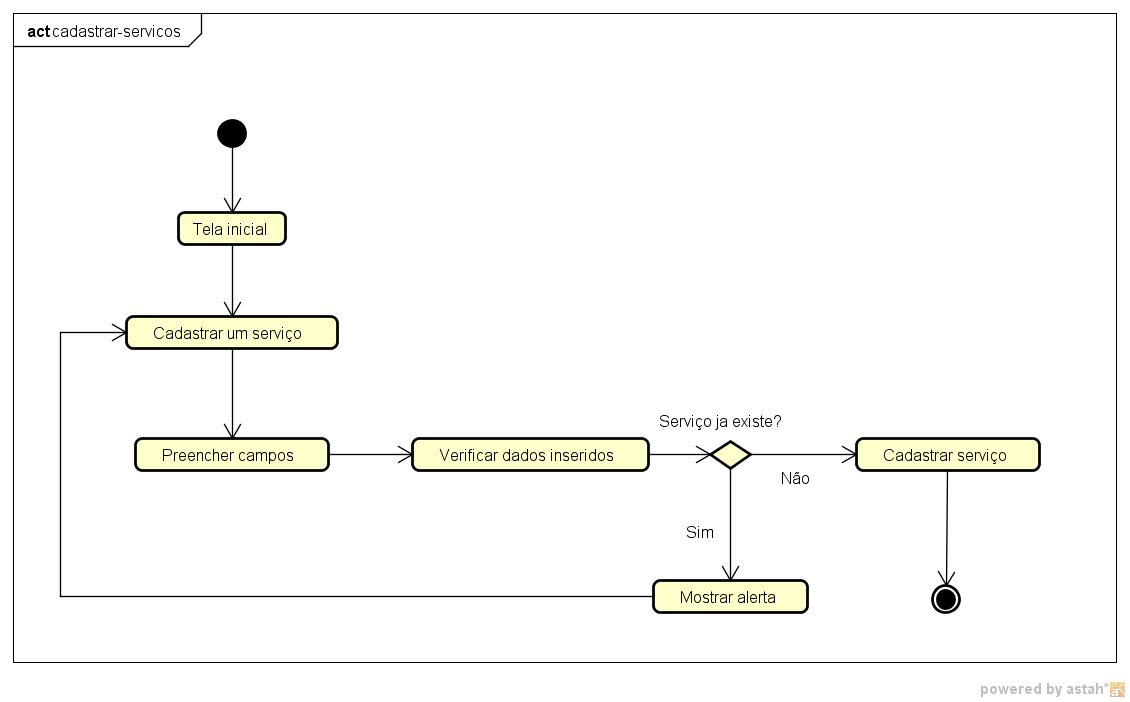
\includegraphics[width=0.8\linewidth]{imagens/servicos.png}
	\end{center}
\end{figure}

\newpage
\subsubsection{CADASTRAR CLIENTE}
\begin{figure}[htb]
	\caption{\label{fig_cadastro} Diagrama de Atividades - Cadastro do Sistema}
	\begin{center}
	    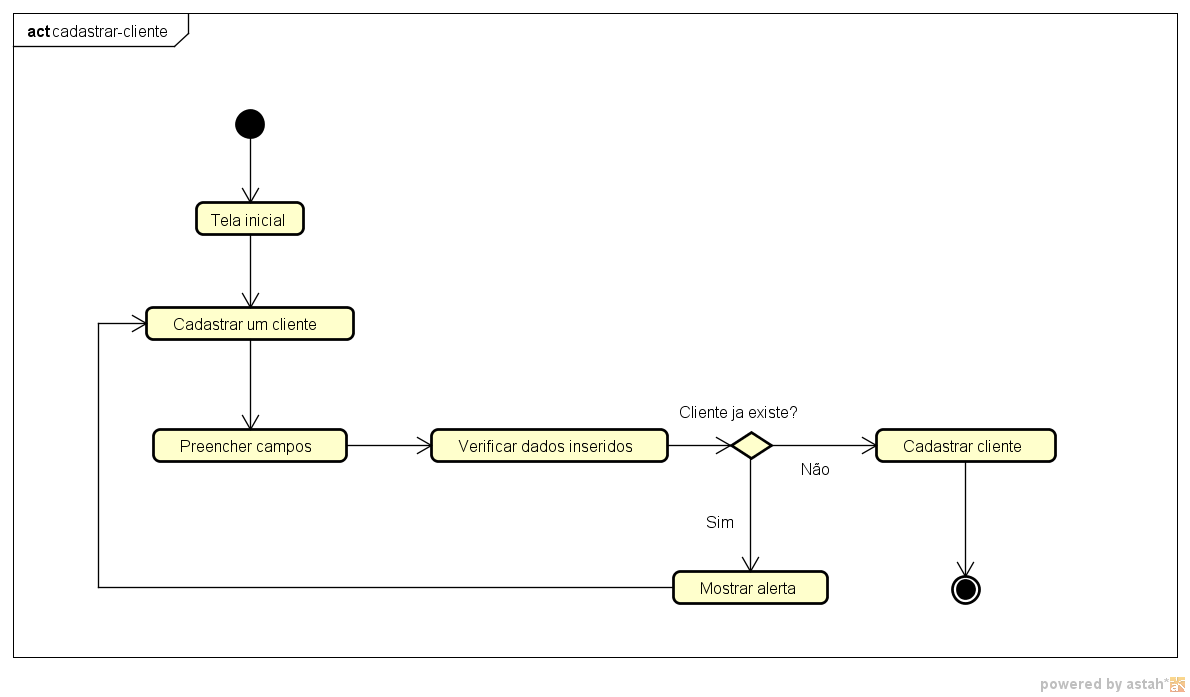
\includegraphics[width=0.8\linewidth]{imagens/cliente.png}
	\end{center}
\end{figure}

\subsubsection{CADASTRAR ORDEM DE SERVIÇO}
\begin{figure}[htb]
	\caption{\label{fig_cadastro} Diagrama de Atividades - Cadastro do Sistema}
	\begin{center}
	    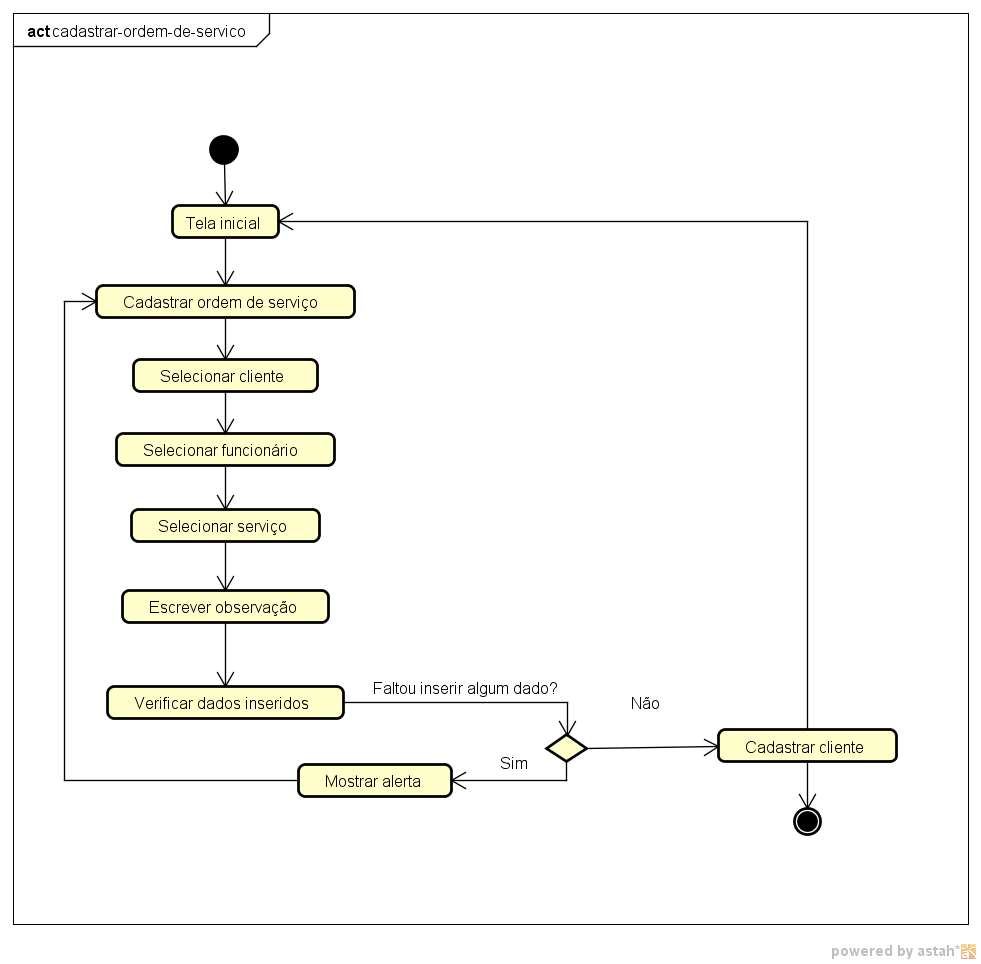
\includegraphics[width=0.6\linewidth]{imagens/ordem-de-servico.png}
	\end{center}
\end{figure}

\newpage
\section{DIAGRAMA DE ENTIDADE RELACIONAMENTO}
\begin{figure}[htb]
	\caption{\label{fig_diagrama-erd} Diagrama de Entidade Relacionamento}
	\begin{center}
	    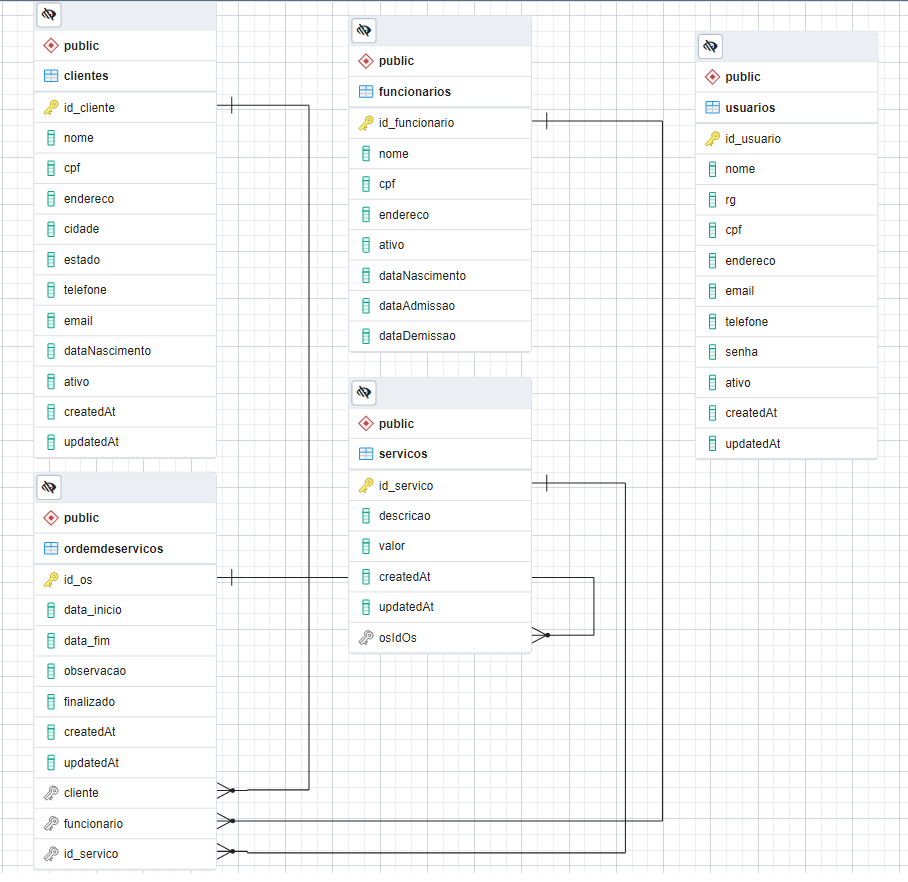
\includegraphics[width=0.8\linewidth]{imagens/diagrama_ERD.png}
	\end{center}
\end{figure}

\newpage
\section{DIAGRAMA DE CLASSES}
\begin{figure}[htb]
	\caption{\label{fig_diagrama-classes} Diagrama de Classes}
	\begin{center}
	    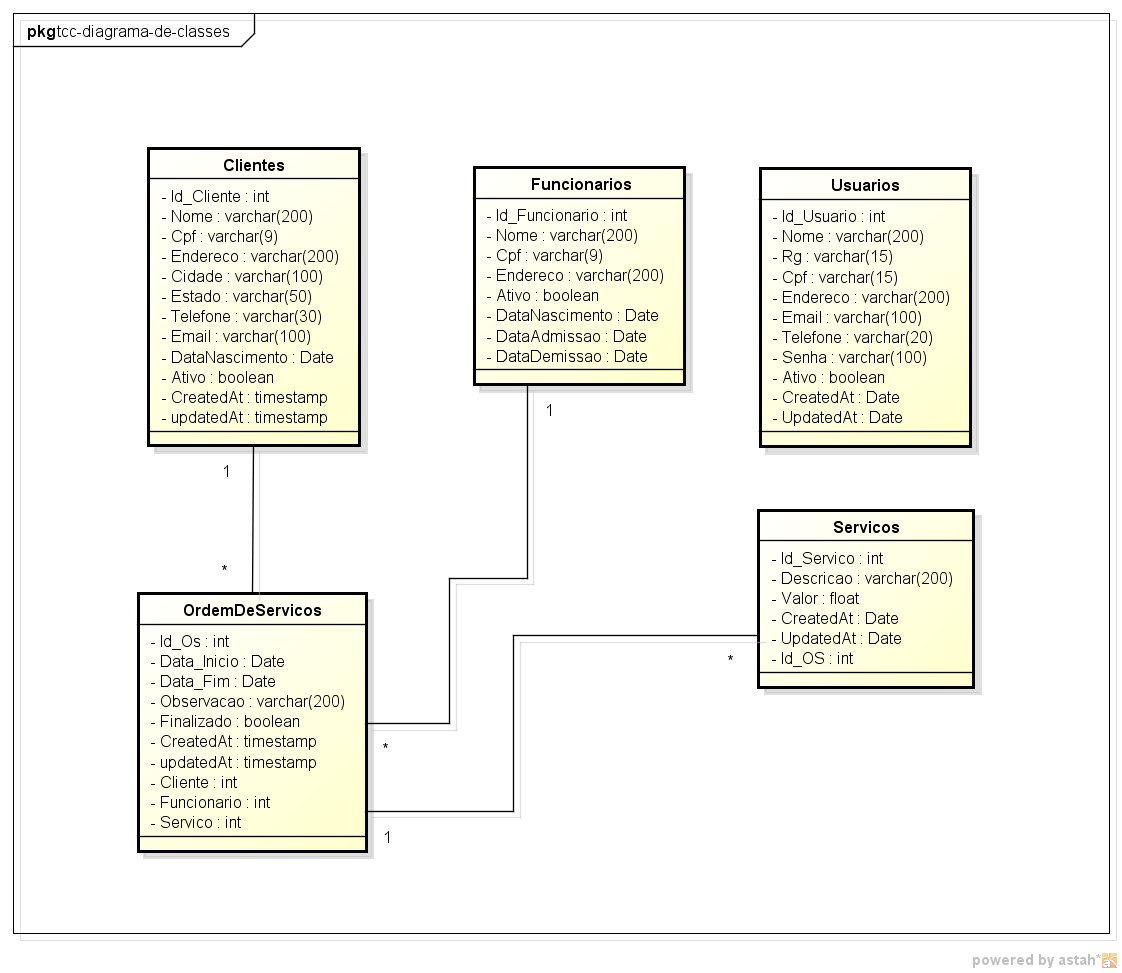
\includegraphics[width=1\linewidth]{imagens/diagrama-de-classes.png}
	\end{center}
\end{figure}

\newpage
\section{DICIONÁRIO DE DADOS}
O dicionário de dados é um documento que descreve, de forma estruturada, o significado, origem, relacionamento e uso dos dados.
\subsection{ENTIDADE DE CLIENTES}
\begin{figure}[htb]
	\begin{center}
	    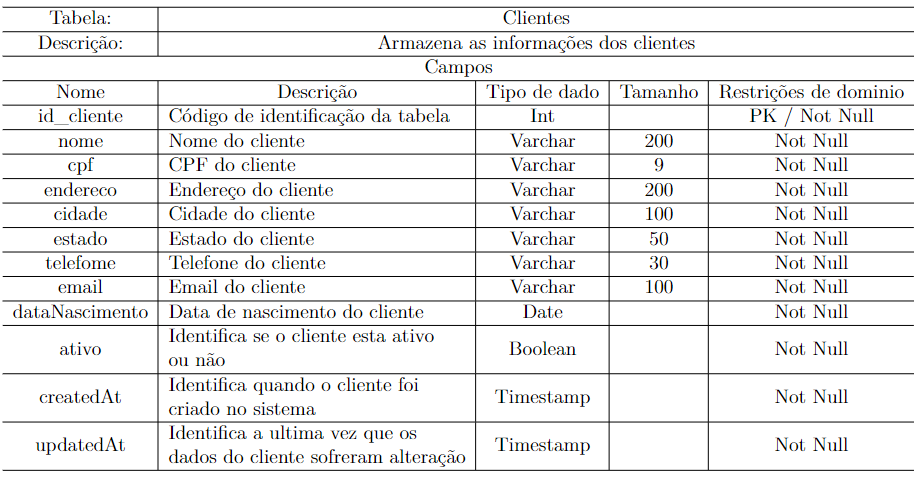
\includegraphics[width=1\linewidth]{imagens/dc1.png}
	\end{center}
\end{figure}

\subsection{ENTIDADE DE FUNCIONÁRIOS}
\begin{figure}[htb]
	\begin{center}
	    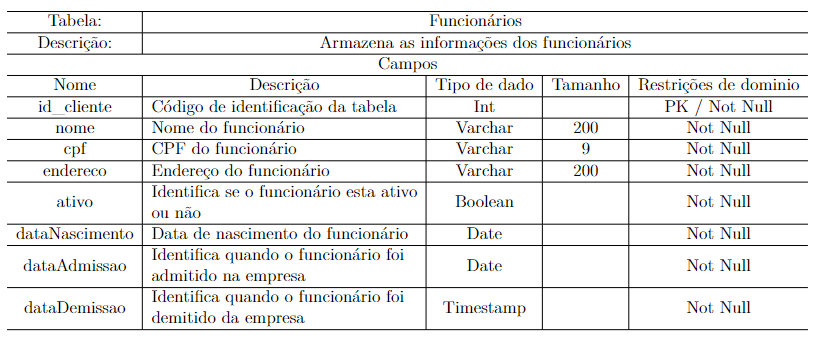
\includegraphics[width=1\linewidth]{imagens/dc2.png}
	\end{center}
\end{figure}

\newpage

\subsection{ENTIDADE DE ORDEM DE SERVIÇO}
\begin{figure}[htb]
	\begin{center}
	    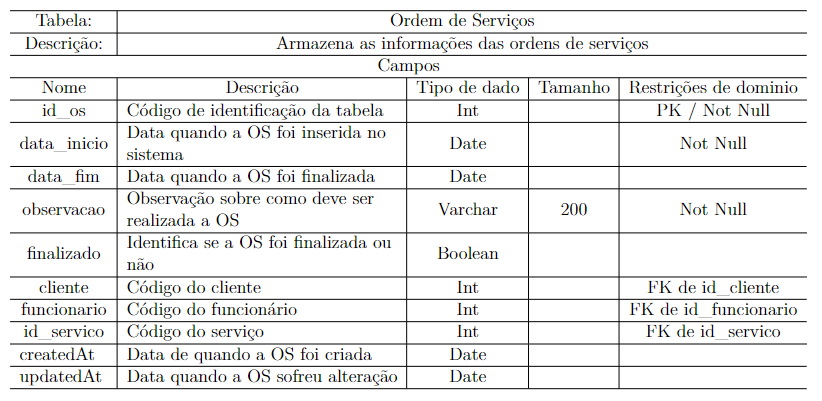
\includegraphics[width=1\linewidth]{imagens/dc3.png}
	\end{center}
\end{figure}


\subsection{ENTIDADE DE SERVIÇOS}
\begin{figure}[htb]
	\begin{center}
	    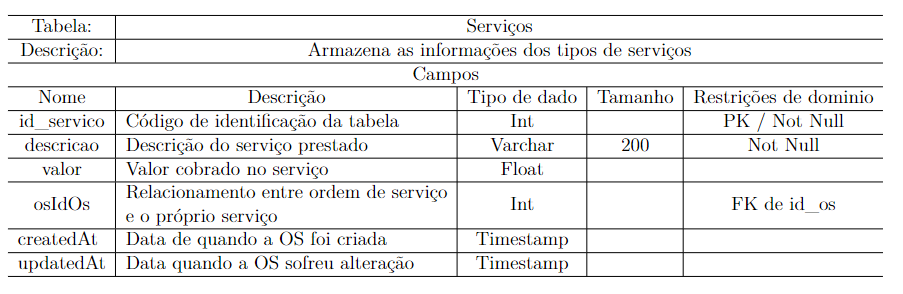
\includegraphics[width=1\linewidth]{imagens/dc4.png}
	\end{center}
\end{figure}

\newpage
\subsection{ENTIDADE DE ORDEM USUÁRIOS}
\begin{figure}[htb]
	\begin{center}
	    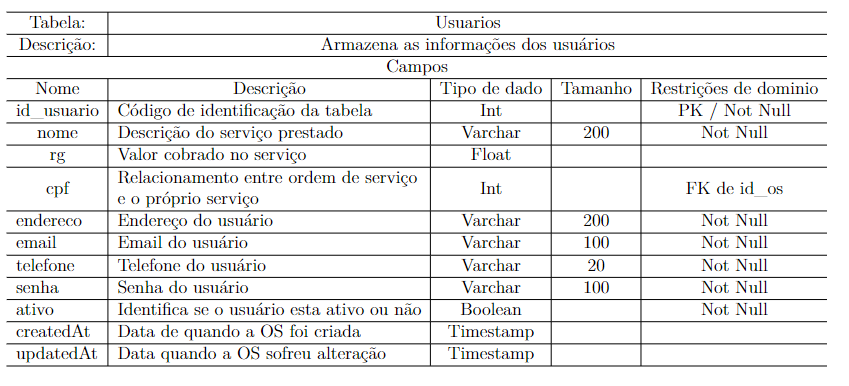
\includegraphics[width=1\linewidth]{imagens/dc5.png}
	\end{center}
\end{figure}


\newpage
\section{TELAS DO SISTEMA}
\subsection{TELA DE LOGIN}
A figura a seguir é a primeira tela ao abrir o aplicativo, nela contém o logo da empresa, os campos para inserir o email e senha do usuário e logo abaixo tem os botões para entrar no sistema e cadastrar um novo usuário.
\begin{figure}[htb]
	\caption{\label{fig_diagrama-classes} Tela de Login}
	\begin{center}
	    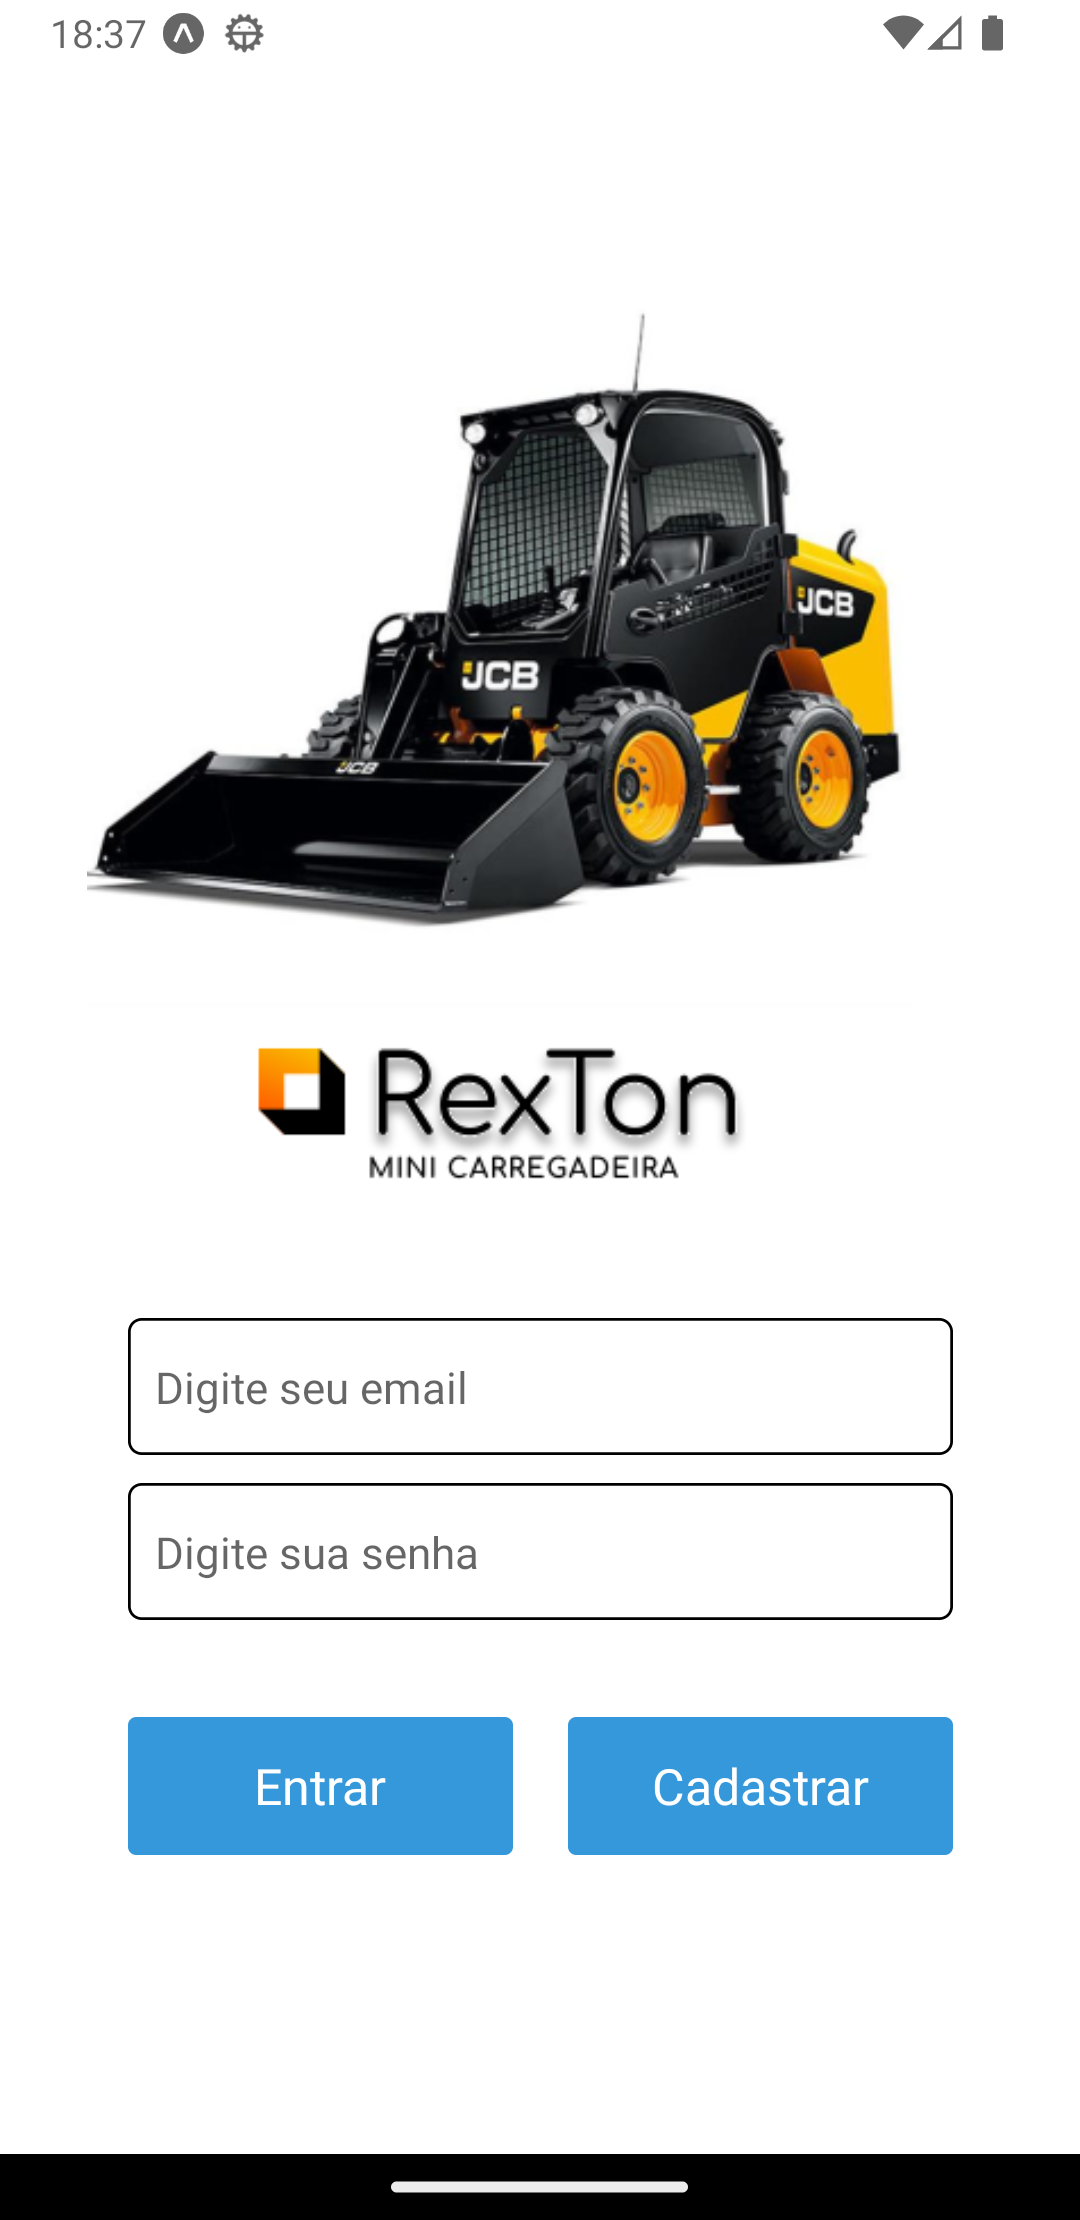
\includegraphics[width=0.5\linewidth]{imagens/login.png}
	\end{center}
\end{figure}

\newpage

\subsection{TELA CADASTRAR USUÁRIOS}
A figura a seguir é por onde é realizado o cadastro de um usuário, cadastro esse que será utilizado na tela anterior para realizar o login no sistema.
\begin{figure}[htb]
	\caption{\label{fig_diagrama-classes} Cadastrar USUÁRIOS}
	\begin{center}
	    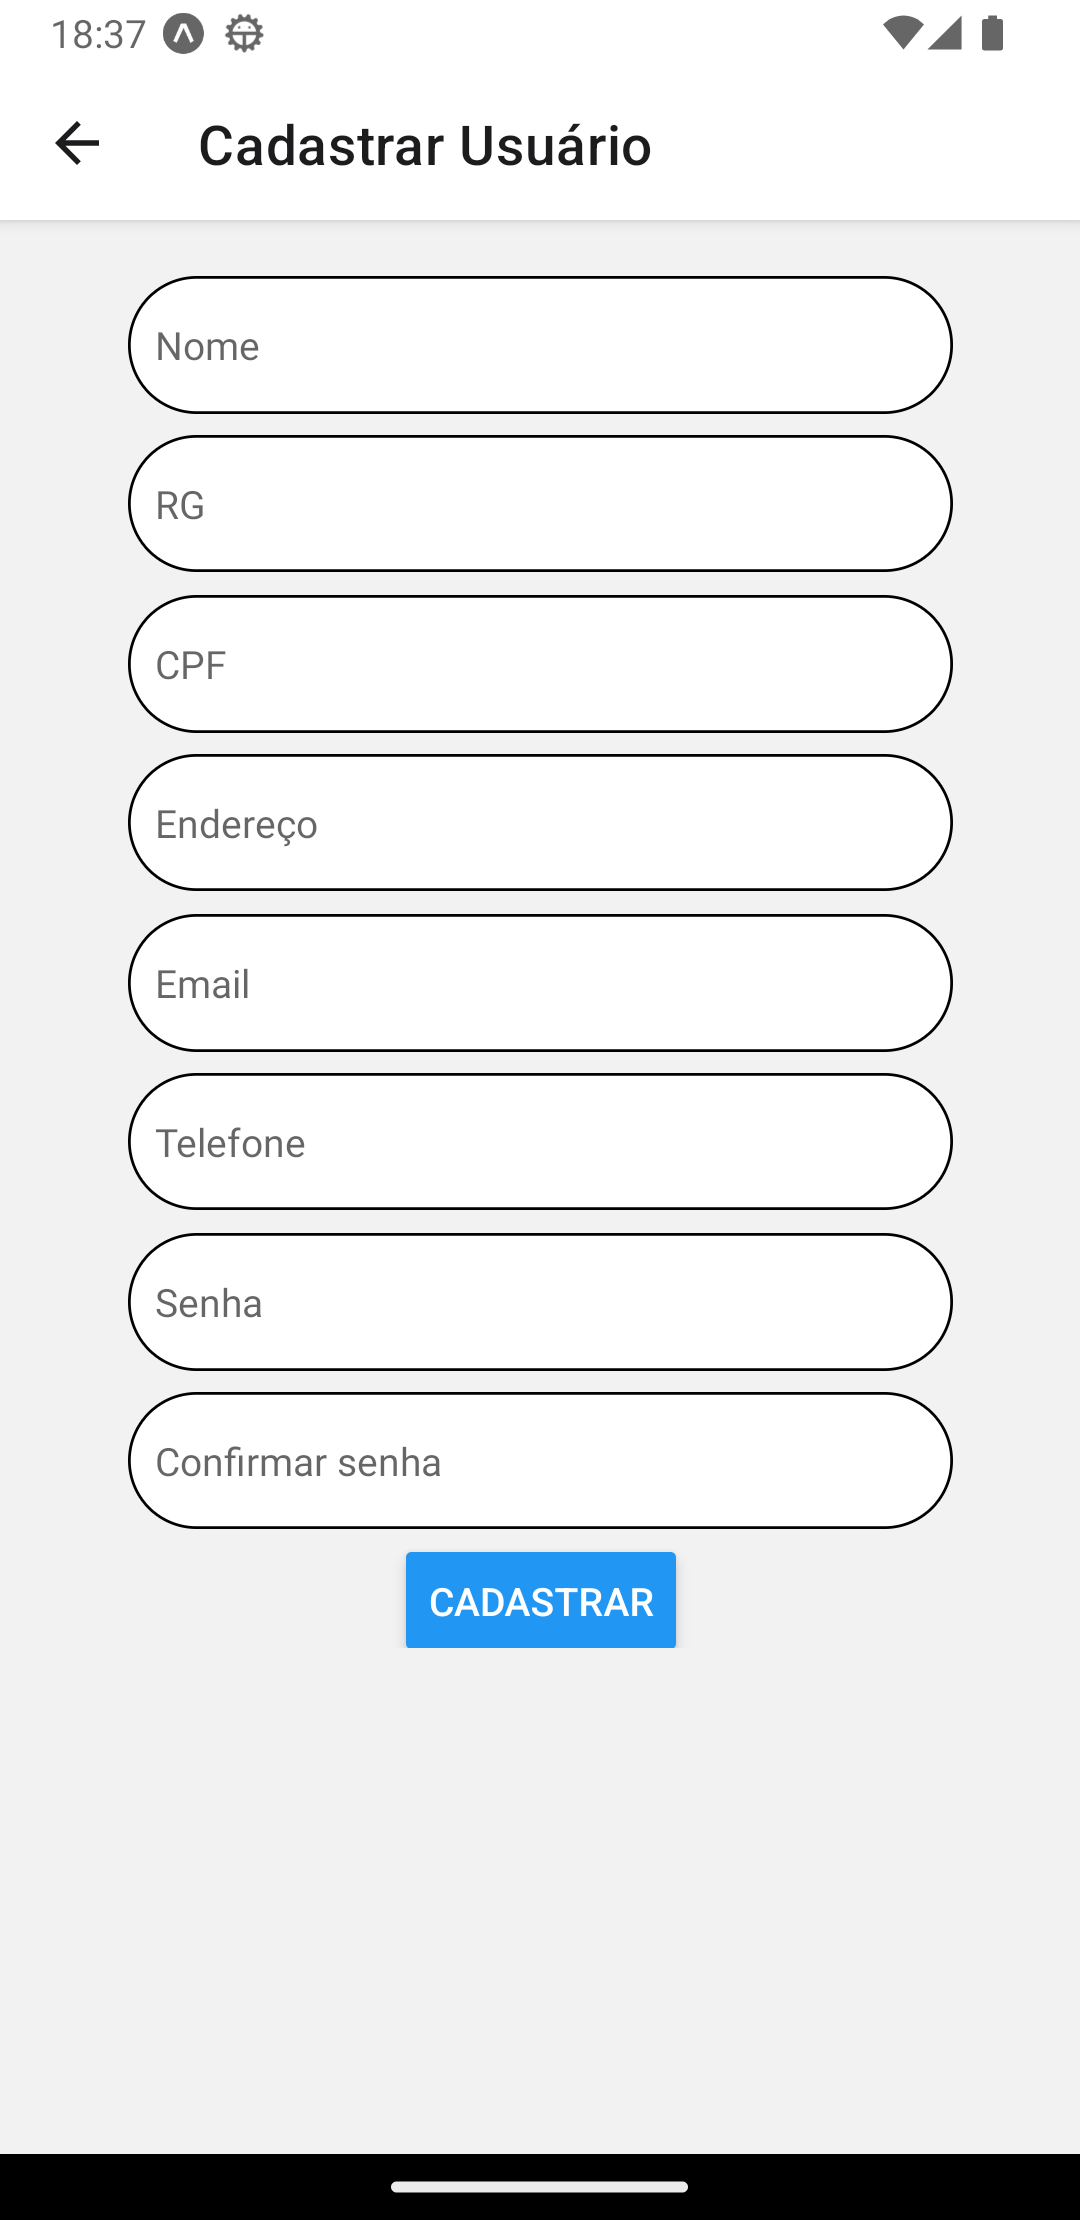
\includegraphics[width=0.5\linewidth]{imagens/tela-cadastrar-usuario.png}
	\end{center}
\end{figure}

\newpage

\subsection{LISTAGEM DE ORDEM DE SERVIÇO}
A figura a seguir é a tela inicial após o usuário realizar o login no sistema, nela contém a listagem das ordens de serviços cadastradas, um botão para cadastrar uma nova OS e no rodapé contém a navegação para outras telas.
\begin{figure}[htb]
	\caption{\label{fig_diagrama-classes} Listagem de OS}
	\begin{center}
	    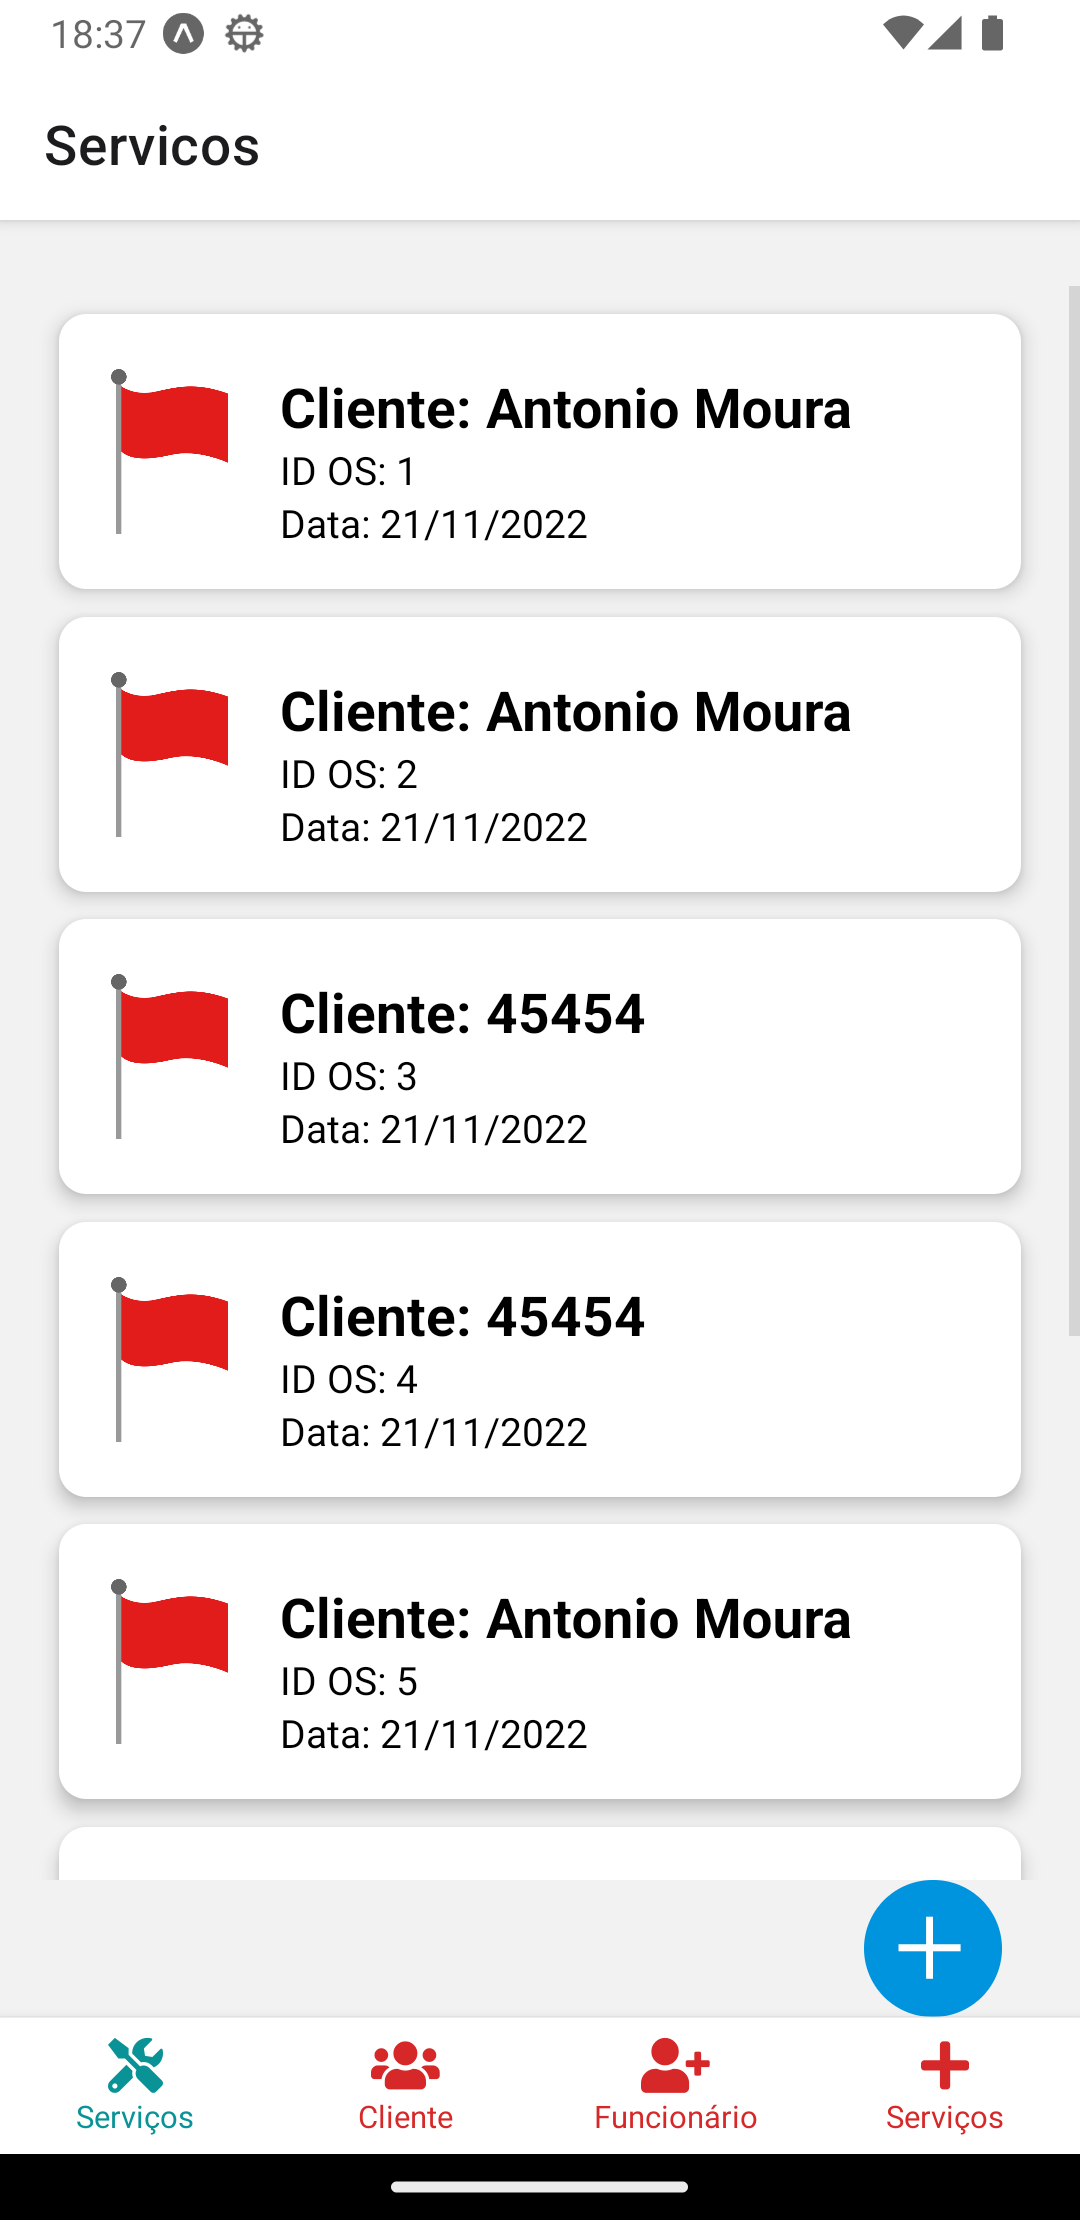
\includegraphics[width=0.5\linewidth]{imagens/listagemOS.png}
	\end{center}
\end{figure}

\newpage

\subsection{TELA CADASTRAR ORDEM DE SERVIÇO}
A figura a seguir contém a tela para realizar de fato o cadastro da ordem de serviço.
\begin{figure}[htb]
	\caption{\label{fig_diagrama-classes} Cadastrar ORDEM DE SERVIÇO}
	\begin{center}
	    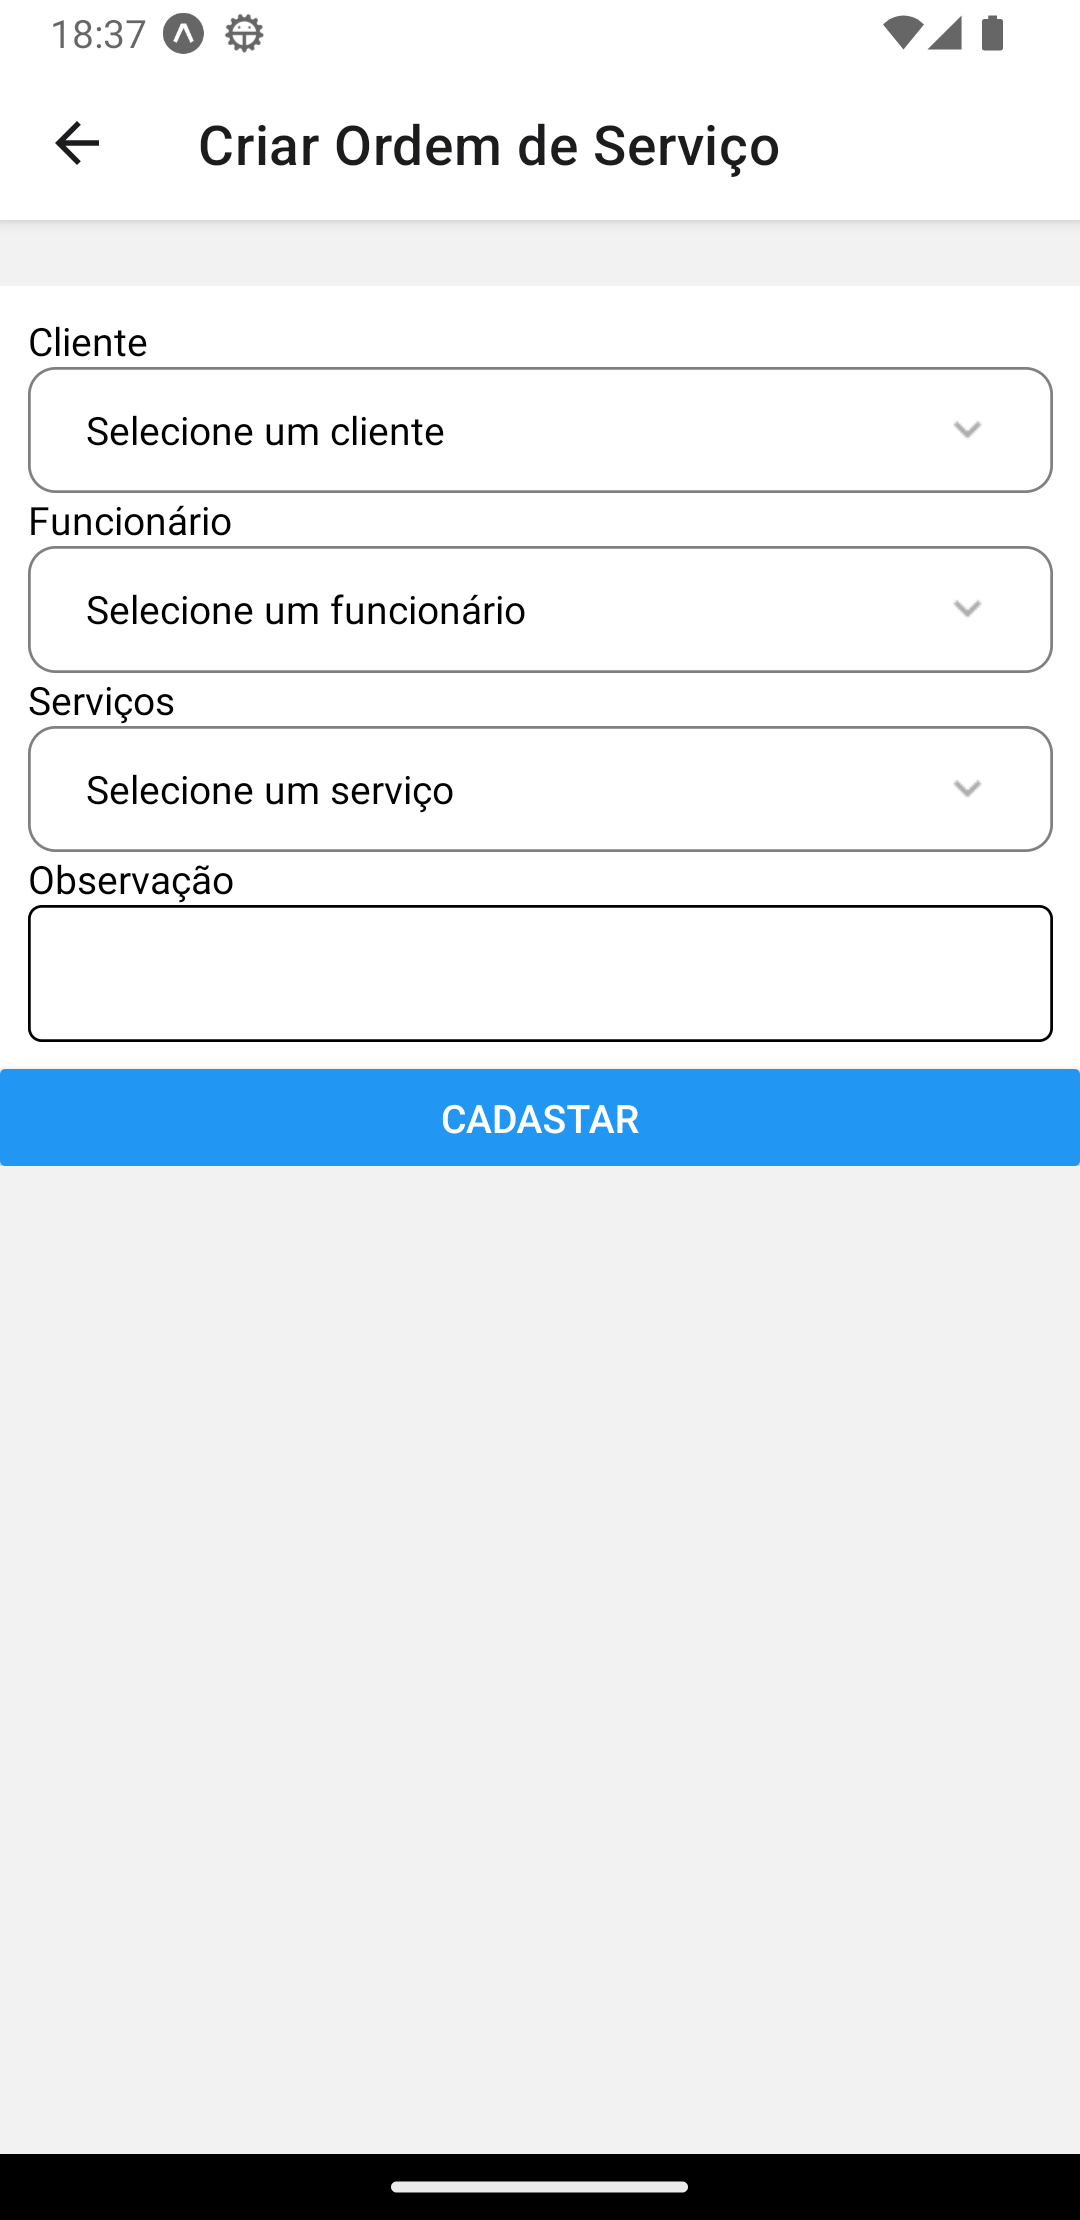
\includegraphics[width=0.5\linewidth]{imagens/criar-OS.png}
	\end{center}
\end{figure}

\newpage

\subsection{TELA CADASTRAR CLIENTES}
A figura a seguir contém a tela para realizar o cadastro de um cliente, informação essa que será utilizada para criar a OS.
\begin{figure}[htb]
	\caption{\label{fig_diagrama-classes} Cadastrar Clientes}
	\begin{center}
	    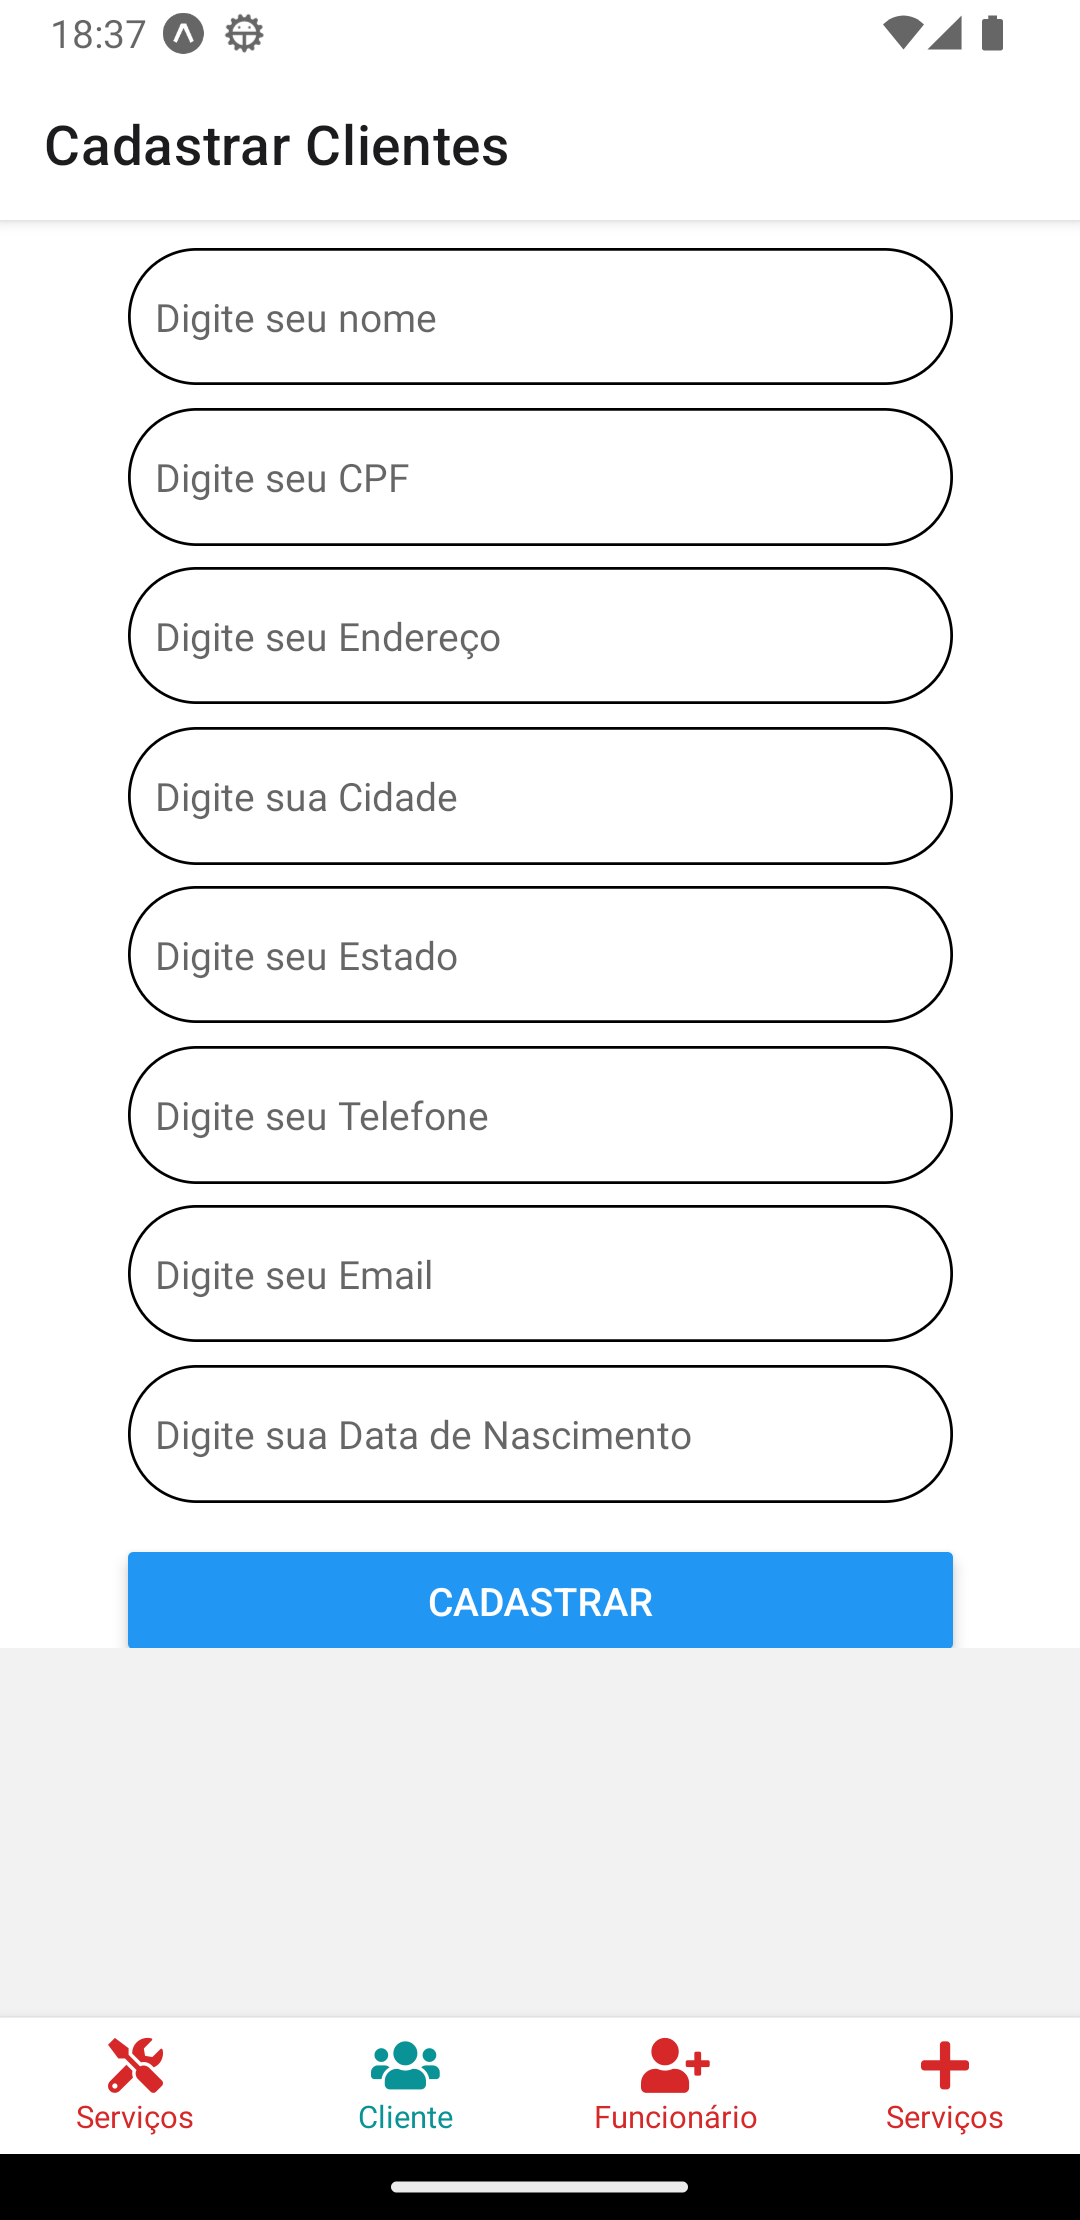
\includegraphics[width=0.5\linewidth]{imagens/tela-cadastrar-cliente.png}
	\end{center}
\end{figure}

\newpage

\subsection{TELA CADASTRAR FUNCIONÁRIO}
A figura a seguir contém a tela para realizar o cadastro de um funcionário, informação essa que será utilizada para criar a OS e que deve identificar qual funcionário realizou a ordem de serviço.
\begin{figure}[htb]
	\caption{\label{fig_diagrama-classes} Cadastrar Funcionário}
	\begin{center}
	    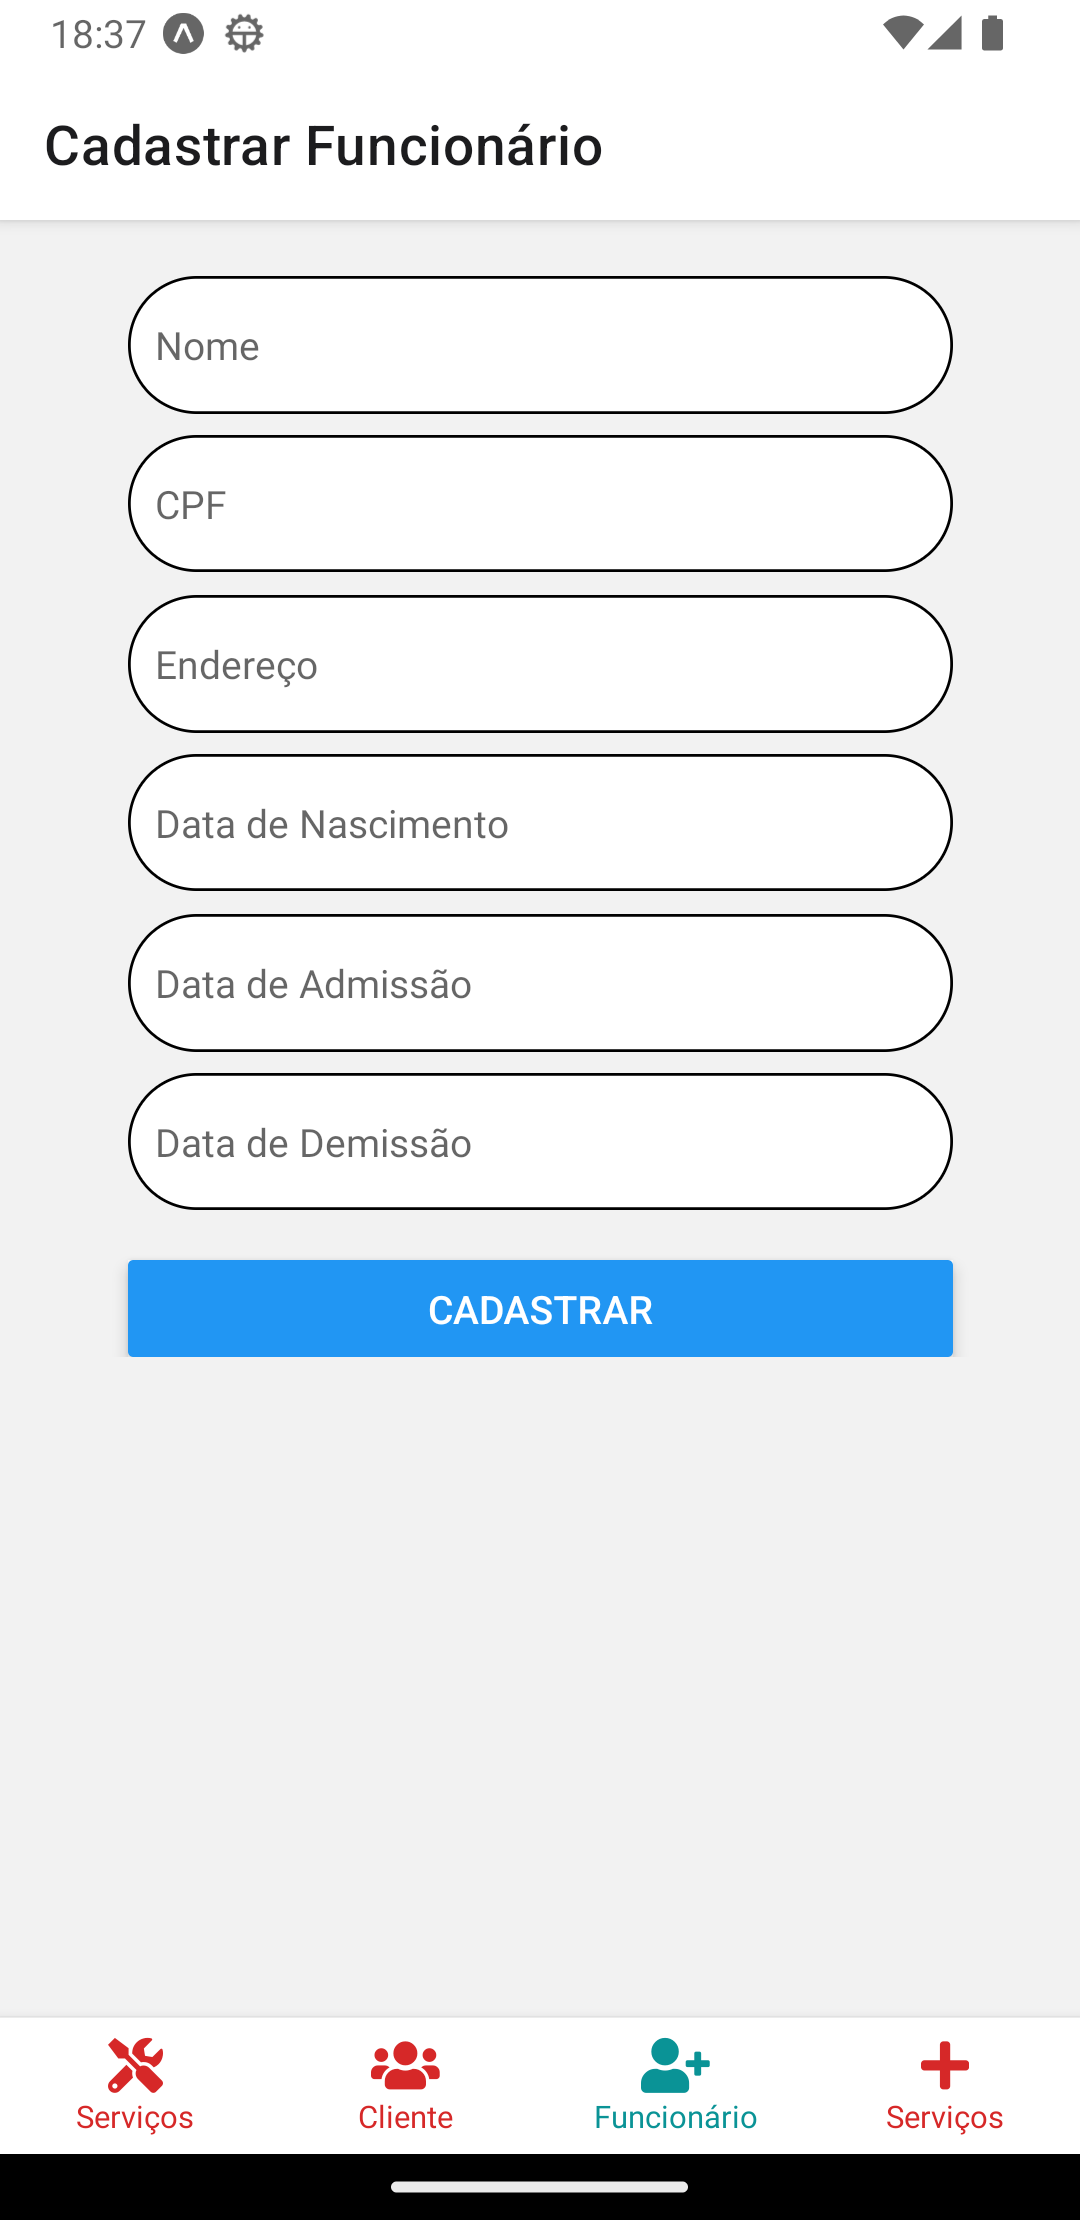
\includegraphics[width=0.5\linewidth]{imagens/tela-cadastrar-funcionario.png}
	\end{center}
\end{figure}

\newpage

\subsection{TELA CADASTRAR TIPOS DE SERVIÇOS}
A figura a seguir é a tela onde se cadastrar o serviço prestado pela empresa e que será utilizada para criação da OS.
\begin{figure}[htb]
	\caption{\label{fig_diagrama-classes} Cadastrar Tipos de Serviços}
	\begin{center}
	    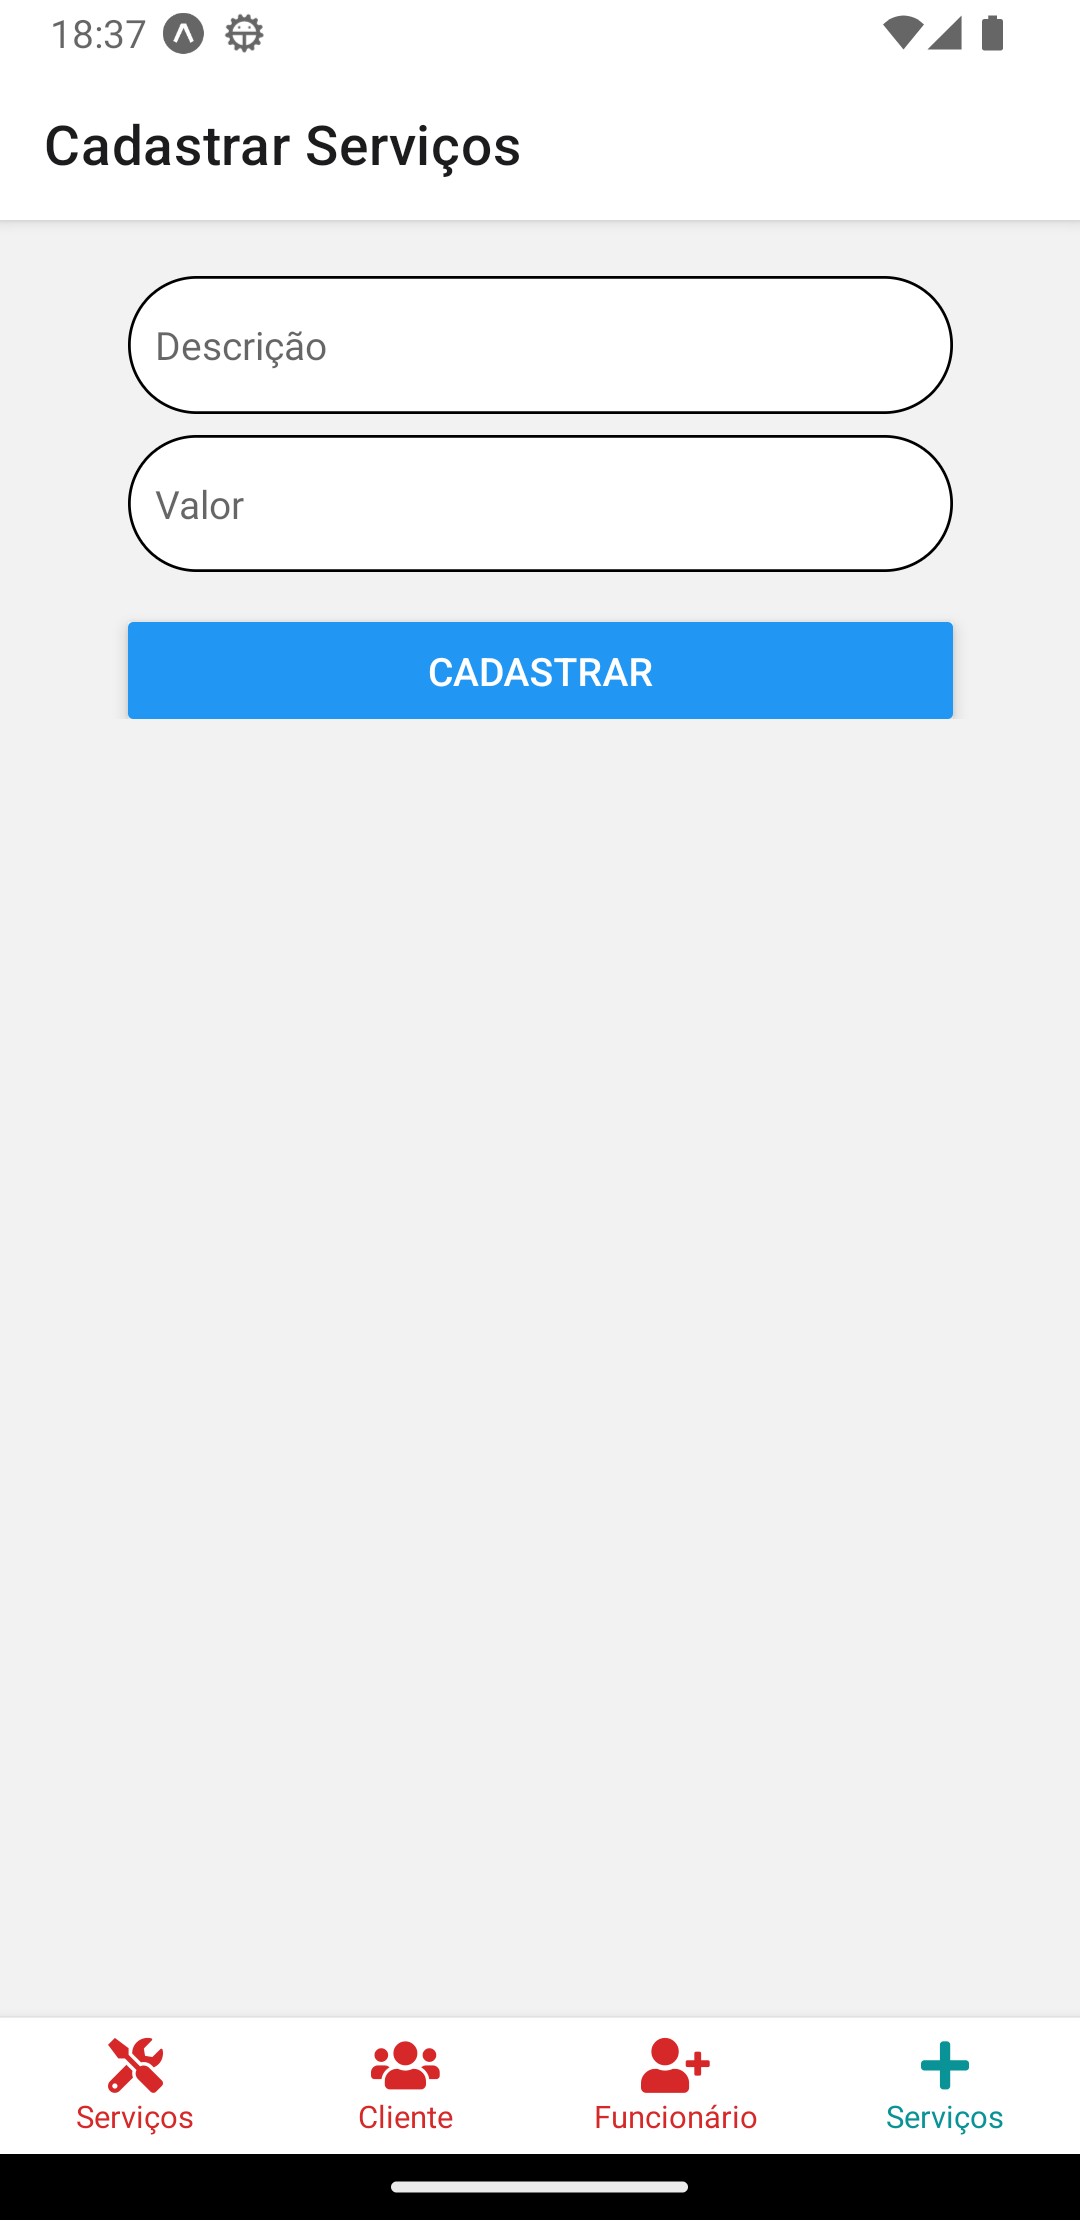
\includegraphics[width=0.5\linewidth]{imagens/tela-cadastrar-servico.png}
	\end{center}
\end{figure}

\newpage

\section{LEVANTAMENTO DE INFORMAÇÕES}
Este trabalho inclui o desenvolvimento de um sistema de gestão das ordens de serviço da empresa. O sistema não possui módulo financeiro, pois foi decidido neste momento utilizar o sistema apenas para os processos internos da empresa. O sistema possui algumas funções importantes para atender ordens de serviço, como consultar clientes, serviços, consultar histórico de fluxo de caixa \cite{caixa} e relatórios. Com este sistema, o processo será mais flexível e preciso. Por exemplo, citando o processo de consulta de uma ordem de serviço a pedido do cliente:

a) com o sistema anterior o atendente pesquisava manualmente no arquivo até encontrar o formulário do cliente, o que geralmente demandava de muito tempo pois existem vários formulários no arquivo;

b) com o sistema desenvolvido o atendente pode efetuar a pesquisa no sistema, ou pelo número da ordem de serviço ou pelo nome do cliente, e o sistema retorna as informações da ordem de serviço. 

O sistema permite publicar vários relatórios para gestão, nos quais podem ser destacados relatórios, ordens de serviço abertas, ordens de serviço fechadas, ordens de serviço do cliente. Com esses relatórios, as empresas podem gerenciar adequadamente as ordens de serviço e tomar decisões quando necessário. O sistema anterior não tinha nenhum tipo de organização de relatório, tudo o que existia era o arquivamento de um formulário impresso. É difícil criar um relatório a partir deste arquivo, pois tem que ser feito manualmente, registrando as ordens de serviço uma a uma. Portanto, é difícil tomar uma decisão porque a informação não está prontamente disponível.

Outra dificuldade do sistema é calcular o orçamento da ordem de serviço. Após o técnico passar o formulário para o atendente, o orçamento da ordem de serviço deve ser calculado manualmente. Para isso, o atendente deve consultar o catálogo impresso para verificar os preços das peças e serviços, que são calculados automaticamente caso o sistema tenha sido desenvolvido e as peças e serviços tiverem sido cadastrados corretamente no sistema.
\\
\\

\section{LEVANTAMENTO DE REQUISITOS}
Este trabalho consiste no desenvolvimento de um sistema mobile, para efetuar o gerenciamento das ordens de serviço da empresa. O sistema não
possui um módulo fiscal, pois neste momento decidiu-se somente a utilização do sistema para
processos internos da empresa.  O sistema possui quatro funcionalidades principais para atender
a ordem de serviço, o cliente, os serviços e os relatórios.
\subsection{ENTREVISTA REALIZADA NA EMPRESA}
\\
a) Qual é o ramo da Empresa?

\linebreak
R: A empresa atua na coleta, remoção e transporte entulho, gestão de estações de transferência de lixo, coleta de entulhos e refugos de obras e demolições, retirada de entulhos após o término das obras, serviços de limpeza urbana.
\\
\\
b) Quais são as pessoas que fazem parte da empresa Rexton?

\linebreak
R: Somente uma pessoa, o proprietário (Tiago)
\\
\\
c) Qual o problema gerado pela falta de um Sistema de Ordem de Serviço?

\linebreak
R: Devido à falta de um software de controle de Ordem de Serviço, não se tem controle dos serviços e reparos executados nos equipamentos da empresa.
\\
\\
d) Qual seria o resultado esperado após a implantação do Sistema de Ordem de Serviço?

\linebreak
R: Com a implantação do Sistema de Ordem de Serviço espera- se que se tenha agilidade, praticidade, maior controle dos materiais gastos, e das atividades rotineiras realizadas na empresa e no arquivamento dos dados de uma forma segura e de fácil acesso.
\\
\\